
%% Optics Questions used on the
%% NYSED Physics Regents Examination
%%--------------------------------------------------

%% this section contains 100 problems

%% NOTE: Jan2002 is the last exam to include geometric optics


%% Section Jan2002
%%--------------------
\element{nysed}{
\begin{question}{Jan2002-Q86}
    The diagram below shows the letter $P$ in front of a plane mirror.
    \begin{center}
    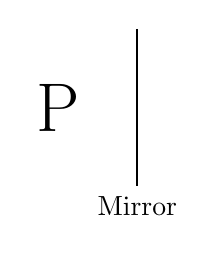
\begin{tikzpicture}
        \draw[thick] (0,1) -- (0,-1) node[anchor=north] {Mirror};
        \node[font=\Huge] at (-1,0) {P};
    \end{tikzpicture}
    \end{center}
    Which diagram best represents the image of $P$ produced by the plane mirror?
    \begin{multicols}{2}
    \begin{choices}
        \AMCboxDimensions{down=-1.0cm}
        \wrongchoice{
            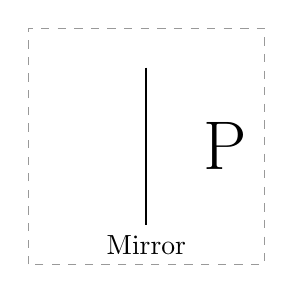
\begin{tikzpicture}
                \draw[dashed,white!60!black] (-1.5,-1.5) rectangle (1.5,1.5);
                \draw[thick] (0,1) -- (0,-1) node[anchor=north] {Mirror};
                \node[font=\Huge] at (1,0) {P};
            \end{tikzpicture}
        }
        \wrongchoice{
            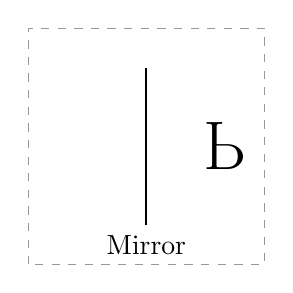
\begin{tikzpicture}
                \draw[dashed,white!60!black] (-1.5,-1.5) rectangle (1.5,1.5);
                \draw[thick] (0,1) -- (0,-1) node[anchor=north] {Mirror};
                \node[font=\Huge,yscale=-1] at (1,0) {P};
            \end{tikzpicture}
        }
        \wrongchoice{
            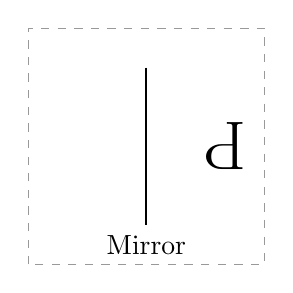
\begin{tikzpicture}
                \draw[dashed,white!60!black] (-1.5,-1.5) rectangle (1.5,1.5);
                \draw[thick] (0,1) -- (0,-1) node[anchor=north] {Mirror};
                \node[font=\Huge,rotate=180] at (1,0) {P};
            \end{tikzpicture}
        }
        \correctchoice{
            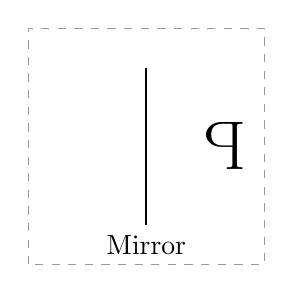
\begin{tikzpicture}
                \draw[dashed,white!60!black] (-1.5,-1.5) rectangle (1.5,1.5);
                \draw[thick] (0,1) -- (0,-1) node[anchor=north] {Mirror};
                \node[font=\Huge,xscale=-1] at (1,0) {P};
            \end{tikzpicture}
        }
    \end{choices}
    \end{multicols}
\end{question}
}

\element{nysed}{
\begin{question}{Jan2002-Q87}
    A student stands \SI{2.0}{\meter} in front of a vertical plane mirror.
    As the student walks toward the mirror, the image:
    \begin{choices}
        \wrongchoice{decreases in size and remains virtual}
        \wrongchoice{decreases in size and remains real}
      \correctchoice{remains the same size and remains virtual}
        \wrongchoice{remains the same size and remains real}
    \end{choices}
\end{question}
}

\element{nysed}{
\begin{question}{Jan2002-Q88}
    An incident light ray travels parallel to the principal axis of a concave spherical mirror.
    After reflecting from the mirror,
        the light ray will travel:
    \begin{choices}
      \correctchoice{through the mirror's principal focus.}
        \wrongchoice{through the mirror's center of curvature.}
        \wrongchoice{parallel to the mirror's principal axis.}
        \wrongchoice{normal to the mirror's principal axis.}
    \end{choices}
\end{question}
}

\element{nysed}{
\begin{question}{Jan2002-Q89}
    The focal length of a concave spherical mirror is \SI{0.060}{\meter}.
    What is the radius of curvature of the mirror?
    \begin{multicols}{2}
    \begin{choices}
        \wrongchoice{\SI{0.060}{\meter}}
      \correctchoice{\SI{0.12}{\meter}}
        \wrongchoice{\SI{8.3}{\meter}}
        \wrongchoice{\SI{17}{\meter}}
    \end{choices}
    \end{multicols}
\end{question}
}

\element{nysed}{
\begin{question}{Jan2002-Q90}
    An image that is \SI{1.0e-2}{\meter} tall is formed on a screen behind a converging lens when an object \SI{2.0}{\meter} tall is placed \SI{8.0}{\meter} in front of the lens.
    What is the distance from the lens to the screen?
    \begin{multicols}{2}
    \begin{choices}
        \wrongchoice{\SI{2.5e-3}{\meter}}
      \correctchoice{\SI{4.0e-2}{\meter}}
        \wrongchoice{\SI{2.5e-1}{\meter}}
        \wrongchoice{\SI{4.0e-1}{\meter}}
    \end{choices}
    \end{multicols}
\end{question}
}

\element{nysed}{
\begin{question}{Jan2002-Q91}
    The diagram below shows an object placed between 1 and 2 focal lengths from a converging lens.
    \begin{center}
    \begin{tikzpicture}
        \draw (-4,0) -- (4,0);
        %% labels
        \foreach \x/\y in {-4/2F,-2/F,2/F,4/2F}
            \fill (\x,0) circle (1.5pt) node[anchor=north] {$\y$};
        %% object
        \draw[very thick,->] (-3,0) -- (-3,1) node[anchor=south] {Object};
        %% lens 1.5 cm tall
        \draw (-0.190,0) arc (180:165.5:6) node[anchor=south] {Converging lens};
        \draw (-0.190,0) arc (180:194.5:6);
        \draw (+0.190,0) arc (0:14.5:6);
        \draw (+0.190,0) arc (360:345.5:6);
    \end{tikzpicture}
    \end{center}
    The image of the object produced by the lens if:
    \begin{choices}
      \correctchoice{real and inverted.}
        \wrongchoice{virtual and inverted.}
        \wrongchoice{real and erect.}
        \wrongchoice{virtual and erect.}
    \end{choices}
\end{question}
}

\element{nysed}{
\begin{question}{Jan2002-Q92}
    The focal length of a lens is not dependent on the:
    \begin{choices}
        \wrongchoice{material from which the lens is made.}
        \wrongchoice{color of the light incident on the lens.}
      \correctchoice{distance of an object from the lens.}
        \wrongchoice{shape or curvature of the lens.}
    \end{choices}
\end{question}
}

\element{nysed}{
\begin{question}{Jan2002-Q93}
    An object is placed \SI{0.20}{\meter} from a converging lens having a focal length of \SI{0.40}{\meter}.
    The distance of the image from the lens is:
    \begin{multicols}{2}
    \begin{choices}
        \wrongchoice{\SI{0.033}{\meter}}
      \correctchoice{\SI{0.050}{\meter}}
        \wrongchoice{\SI{0.16}{\meter}}
        \wrongchoice{\SI{0.20}{\meter}}
    \end{choices}
    \end{multicols}
\end{question}
}

\element{nysed}{
\begin{question}{Jan2002-Q94}
    Images formed by diverging mirrors are always:
    \begin{multicols}{2}
    \begin{choices}
        \wrongchoice{real and inverted.}
        \wrongchoice{real and erect.}
        \wrongchoice{virtual and inverted.}
      \correctchoice{virtual and erect.}
    \end{choices}
    \end{multicols}
\end{question}
}

\element{nysed}{
\begin{question}{Jan2002-Q95}
    Spherical aberration is a defect associated with:
    \begin{choices}
        \wrongchoice{spherical mirrors, only.}
        \wrongchoice{plane mirrors, only.}
      \correctchoice{both spherical mirrors and lenses.}
        \wrongchoice{both plane mirrors and lenses.}
    \end{choices}
\end{question}
}


%% Section June2001
%%--------------------
\element{nysed}{
\begin{question}{June2001-Q86}
    Which diagram best represents image $I$,
        which is formed by placing object $O$ in front of a plane mirror?
    \begin{multicols}{2}
    \begin{choices}
        \AMCboxDimensions{down=-1.0cm}
        \wrongchoice{
            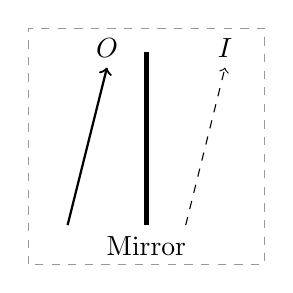
\begin{tikzpicture}
                \draw[dashed,white!60!black] (-1.5,-1.5) rectangle (1.5,1.5);
                \draw[ultra thick] (0,1.2) -- (0,-1) node[anchor=north] {Mirror};
                \draw[thick,->] (-1,-1) -- (-0.5,1) node[anchor=south] {$O$};
                \draw[dashed,->] (+0.5,-1) -- (+1,1) node[anchor=south] {$I$};
            \end{tikzpicture}
        }
        \correctchoice{
            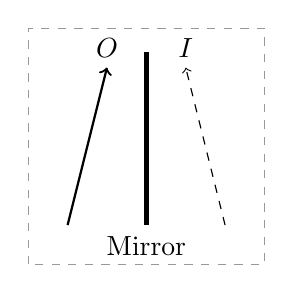
\begin{tikzpicture}
                \draw[dashed,white!60!black] (-1.5,-1.5) rectangle (1.5,1.5);
                \draw[ultra thick] (0,1.2) -- (0,-1) node[anchor=north] {Mirror};
                \draw[thick,->] (-1,-1) -- (-0.5,1) node[anchor=south] {$O$};
                \draw[dashed,->] (+1,-1) -- (+0.5,1) node[anchor=south] {$I$};
            \end{tikzpicture}
        }
        \wrongchoice{
            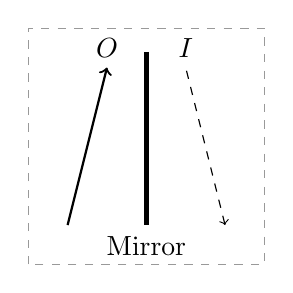
\begin{tikzpicture}
                \draw[dashed,white!60!black] (-1.5,-1.5) rectangle (1.5,1.5);
                \draw[ultra thick] (0,1.2) -- (0,-1) node[anchor=north] {Mirror};
                \draw[thick,->] (-1,-1) -- (-0.5,1) node[anchor=south] {$O$};
                \draw[dashed,<-] (+1,-1) -- (+0.5,1) node[anchor=south] {$I$};
            \end{tikzpicture}
        }
        \wrongchoice{
            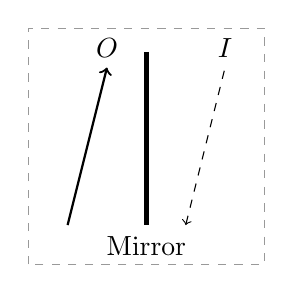
\begin{tikzpicture}
                \draw[dashed,white!60!black] (-1.5,-1.5) rectangle (1.5,1.5);
                \draw[ultra thick] (0,1.2) -- (0,-1) node[anchor=north] {Mirror};
                \draw[thick,->] (-1,-1) -- (-0.5,1) node[anchor=south] {$O$};
                \draw[dashed,<-] (0.5,-1) -- (1,1) node[anchor=south] {$I$};
            \end{tikzpicture}
        }
    \end{choices}
    \end{multicols}
\end{question}
}

\element{nysed}{
\begin{question}{June2001-Q87}
    The diagram below shows an arrow placed in front of a converging lens:
    \begin{center}
    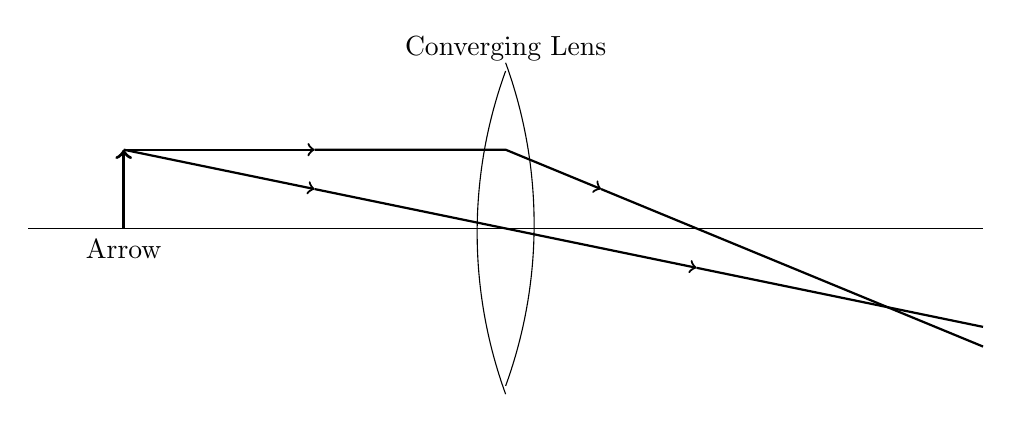
\begin{tikzpicture}[x=0.1\columnwidth]
        %% Lens and Normal Line
        \draw (-5,0) -- (5,0);
        \draw (0,2) arc (160:200:6cm);
        \draw (0,-2) arc (-20:20:6cm);
        \node[anchor=south] at (0,2) {Converging Lens};
        %% Object and Path
        \draw[very thick,->] (-4,0) -- (-4,1)
            node[pos=0.0,anchor=north] {Arrow};
        \draw[thick,->] (-4,1) -- (-2,1);
        \draw[thick,->] (-2,1) -- (0,1) -- (1,0.5);
        \draw[thick] (1,0.5) -- (5,-1.5);
        \draw[thick,->] (-4,1) -- (-2,0.5);
        \draw[thick,->] (-2,0.5) -- (0,0) -- (2,-0.5);
        \draw[thick] (2,-0.5) -- (5,-1.25);
    \end{tikzpicture}
    \end{center}
    The lens forms an image of the arrow that is:
    \begin{multicols}{2}
    \begin{choices}
      \correctchoice{real and inverted}
        \wrongchoice{real and erect}
        \wrongchoice{virtual and inverted}
        \wrongchoice{virtual and erect}
    \end{choices}
    \end{multicols}
\end{question}
}

\element{nysed}{
\begin{question}{June2001-Q88}
    Light rays from a candle flame are incident on a convex mirror.
    After reflecting from the mirror, these light rays:
    \begin{choices}
        \wrongchoice{converge and form a virtual image.}
      \correctchoice{converge and form a real image.}
        \wrongchoice{diverge and form a virtual image.}
        \wrongchoice{diverge and form a real image.}
    \end{choices}
\end{question}
}

\element{nysed}{
\begin{question}{June2001-Q89}
    The diagram below shows an object located at point $P$,
        \SI{0.25}{\meter} from a concave spherical mirror with principal focus $F$.
    The focal length of the mirror is \SI{0.10}{\meter}.
    \begin{center}
    \begin{tikzpicture}
        %% axis
        \draw (-6,0) -- (0,0);
        %% labels
        \fill (-2,0) circle (1.5pt) node[anchor=north] {$F$};
        \fill (-4,0) circle (1.5pt) node[anchor=north] {$P$};
        \draw[very thick,-latex] (-4,0) -- (-4,1);
        %% mirror
        \draw[very thick] (-4,0) ++ (338:4) arc(-22:22:4) node[anchor=south west] {Concave Mirror};
    \end{tikzpicture}
    \end{center}
    How does the image change as the object is moved from point $P$ toward point $F$?
    \begin{choices}
        \wrongchoice{Its distance from the mirror decreases and the size of the image decreases}
      \correctchoice{Its distance from the mirror decreases and the size of the image increases}
        \wrongchoice{Its distance from the mirror increases and the size of the image decreases}
        \wrongchoice{Its distance from the mirror increases and the size of the image increases}
    \end{choices}
\end{question}
}

\element{nysed}{
\begin{question}{June2001-Q90}
    The diagram below shows light ray $R$ incident on a glass lens in air.
    \begin{center}
    \begin{tikzpicture}
        %% NOTE: TODO: draw tikz
    \end{tikzpicture}
    \includegraphics[keepaspectratio,scale=0.50]{June2001-Q90}
    \end{center}
    Which ray best represents the path of light ray $R$ after it passes through the lens?
    \begin{multicols}{4}
    \begin{choices}[o]
      \correctchoice{$A$}
        \wrongchoice{$B$}
        \wrongchoice{$C$}
        \wrongchoice{$D$}
    \end{choices}
    \end{multicols}
\end{question}
}

\element{nysed}{
\begin{question}{June2001-Q91}
    The diagram below shows two parallel rays,
        $X$ and $Y$, approaching a concave spherical mirror.
    \begin{center}
    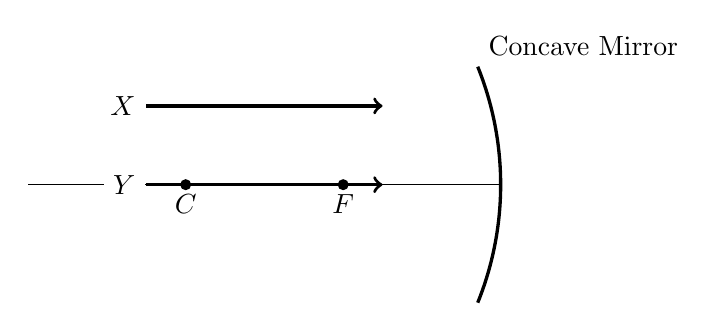
\begin{tikzpicture}
        %% axis
        \draw (-6,0) -- (0,0);
        %% labels
        \fill (-2,0) circle (2pt) node[anchor=north] {$F$};
        \fill (-4,0) circle (2pt) node[anchor=north] {$C$};
        %% rays
        \foreach \x/\y in {0/Y,1/X} \draw[very thick,->] (-4.5,\x) -- ++(0:3) node[pos=0,anchor=east,fill=white] {$\y$};
        %% mirror
        \draw[very thick] (-4,0) ++ (338:4) arc(-22:22:4) node[anchor=south west] {Concave Mirror};
    \end{tikzpicture}
    \end{center}
    Which light will reflect through the mirror's center of curvature, $C$?
    \begin{choices}
        \wrongchoice{ray $X$, only}
      \correctchoice{ray $Y$, only}
        \wrongchoice{both ray $X$ and ray $Y$}
        \wrongchoice{neither ray $X$ nor ray $Y$}
    \end{choices}
\end{question}
}

\element{nysed}{
\begin{question}{June2001-Q92}
    Which optical devices in air can both form real images?
    \begin{choices}
      \correctchoice{concave mirror and convex lens}
        \wrongchoice{concave mirror and concave lens}
        \wrongchoice{plane mirror and convex lens}
        \wrongchoice{plane mirror and concave lens}
    \end{choices}
\end{question}
}

\element{nysed}{
\begin{question}{June2001-Q93}
    An object is located \SI{0.15}{\meter} from a converging lens with focal length \SI{0.10}{\meter}.
    How far from the lens is the image formed?
    \begin{multicols}{2}
    \begin{choices}
        \wrongchoice{\SI{0.060}{\meter}}
        \wrongchoice{\SI{0.10}{\meter}}
        \wrongchoice{\SI{0.15}{\meter}}
      \correctchoice{\SI{0.30}{\meter}}
    \end{choices}
    \end{multicols}
\end{question}
}

\element{nysed}{
\begin{question}{June2001-Q94}
    When a student \SI{1.5}{\meter} tall stands \SI{5.0}{\meter} in front of a lens,
        his image forms on a screen located \SI{0.50}{\meter} behind the lens.
    What is the height of the students image?
    \begin{multicols}{2}
    \begin{choices}
        \wrongchoice{\SI{0.015}{\meter}}
      \correctchoice{\SI{0.15}{\meter}}
        \wrongchoice{\SI{1.5}{\meter}}
        \wrongchoice{\SI{15}{\meter}}
    \end{choices}
    \end{multicols}
\end{question}
}

\element{nysed}{
\begin{question}{June2001-Q95}
    Which phenomena cause chromatic aberration to occur when polychromatic light passes through a lens?
    \begin{choices}
        \wrongchoice{diffraction and refraction}
        \wrongchoice{diffraction and reflection}
      \correctchoice{dispersion and refraction}
        \wrongchoice{dispersion and reflection}
    \end{choices}
\end{question}
}


%% Section Jan2001
%%--------------------
\element{nysed}{
\begin{question}{Jan2001-Q86}
    A converging lens has a focal length of \SI{0.080}{\meter}.
    A light ray travels from the object to the lens parallel to the principal axis.
    \begin{center}
        \includegraphics[keepaspectratio,scale=0.85]{Jan2001-Q86}
    \end{center}
    Which line best represents the path of the ray after it leaves the lens?
    \begin{multicols}{4}
    \begin{choices}
        %% NOTE: A, B, C, D??
        \wrongchoice{1}
        \wrongchoice{2}
      \correctchoice{3}
        \wrongchoice{4}
    \end{choices}
    \end{multicols}
\end{question}
}

\element{nysed}{
\begin{question}{Jan2001-Q87}
    A converging lens has a focal length of \SI{0.080}{\meter}.
    A light ray travels from the object to the lens parallel to the principal axis.
    \begin{center}
        \includegraphics[keepaspectratio,scale=0.85]{Jan2001-Q86}
    \end{center}
    How far from the lens is the image formed?
    \begin{multicols}{2}
    \begin{choices}
        \wrongchoice{\SI{0.020}{\meter}}
        \wrongchoice{\SI{0.18}{\meter}}
      \correctchoice{\SI{0.40}{\meter}}
        \wrongchoice{\SI{0.80}{\meter}}
    \end{choices}
    \end{multicols}
\end{question}
}

\element{nysed}{
\begin{question}{Jan2001-Q88}
    A converging lens has a focal length of \SI{0.080}{\meter}.
    A light ray travels from the object to the lens parallel to the principal axis.
    \begin{center}
        \includegraphics[keepaspectratio,scale=0.85]{Jan2001-Q86}
    \end{center}
    If the lens is made of crown glass,
        the speed of the light in the lens is closest to:
    \begin{multicols}{2}
    \begin{choices}
        \wrongchoice{\SI{1.5e8}{\meter\per\second}}
      \correctchoice{\SI{2.0e8}{\meter\per\second}}
        \wrongchoice{\SI{3.0e8}{\meter\per\second}}
        \wrongchoice{\SI{4.0e8}{\meter\per\second}}
    \end{choices}
    \end{multicols}
\end{question}
}

\element{nysed}{
\begin{question}{Jan2001-Q89}
    A converging lens has a focal length of \SI{0.080}{\meter}.
    A light ray travels from the object to the lens parallel to the principal axis.
    \begin{center}
        \includegraphics[keepaspectratio,scale=0.85]{Jan2001-Q86}
    \end{center}
    Which phenomenon best explains the path of the light through the lens?
    \begin{multicols}{2}
    \begin{choices}
        \wrongchoice{diffraction}
        \wrongchoice{dispersion}
        \wrongchoice{reflection}
      \correctchoice{refraction}
    \end{choices}
    \end{multicols}
\end{question}
}

\element{nysed}{
\begin{question}{Jan2001-Q90}
    A converging lens has a focal length of \SI{0.080}{\meter}.
    A light ray travels from the object to the lens parallel to the principal axis.
    \begin{center}
        \includegraphics[keepaspectratio,scale=0.85]{Jan2001-Q86}
    \end{center}
    If the lens were placed in water,
        its focal length would:
    \begin{multicols}{2}
    \begin{choices}
        \wrongchoice{decrease}
      \correctchoice{increase}
        \wrongchoice{remain the same}
    \end{choices}
    \end{multicols}
\end{question}
}

\element{nysed}{
\begin{question}{Jan2001-Q91}
    Which characteristics best describe the image produced by a plane mirror?
    \begin{choices}
        \wrongchoice{real and inverted}
        \wrongchoice{real and erect}
        \wrongchoice{virtual and inverted}
      \correctchoice{virtual and erect}
    \end{choices}
\end{question}
}

\element{nysed}{
\begin{question}{Jan2001-Q92}
    When an object is placed at the focal point of a concave mirror, the mirror produces:
    \begin{choices}
        \wrongchoice{an image that is smaller than the object}
        \wrongchoice{an image that is larger than the object}
        \wrongchoice{an image that is the same size as the object}
      \correctchoice{no image of the object}
    \end{choices}
\end{question}
}

\element{nysed}{
\begin{question}{Jan2001-Q93}
    Which optical device causes parallel light rays to diverge?
    \begin{multicols}{2}
    \begin{choices}
      \correctchoice{convex mirror}
        \wrongchoice{concave mirror}
        \wrongchoice{plane mirror}
        \wrongchoice{convex lens}
    \end{choices}
    \end{multicols}
\end{question}
}

\element{nysed}{
\begin{question}{Jan2001-Q94}
    When a boy is \SI{1.00}{\meter} tall stands in front of a vertical plane mirror,
        he is able to see the image of his entire body.
    What is the minimum height, from top to bottom, of the mirror?
    \begin{multicols}{2}
    \begin{choices}
        \wrongchoice{\SI{1.00}{\meter}}
        \wrongchoice{\SI{2.00}{\meter}}
      \correctchoice{\SI{0.50}{\meter}}
        \wrongchoice{\SI{0.25}{\meter}}
    \end{choices}
    \end{multicols}
\end{question}
}

\element{nysed}{
\begin{question}{Jan2001-Q95}
    An object arrow is placed in front of a concave mirror having center of curvature $C$ and principal focus $F$.
    Which diagram best shows the location of point $I$,
        the image of the tip of the object arrow?
    \begin{multicols}{2}
    \begin{choices}
        \AMCboxDimensions{down=-1.5em}
        \wrongchoice{\includegraphics[keepaspectratio,scale=0.75]{Jan2001-Q95-A}}
        \wrongchoice{\includegraphics[keepaspectratio,scale=0.75]{Jan2001-Q95-B}}
      \correctchoice{\includegraphics[keepaspectratio,scale=0.75]{Jan2001-Q95-C}}
        \wrongchoice{\includegraphics[keepaspectratio,scale=0.75]{Jan2001-Q95-D}}
    \end{choices}
    \end{multicols}
\end{question}
}


%% Section June2000
%%--------------------
\element{nysed}{
\begin{question}{June2000-Q86}
    A candle is located beyond the principal focus,
        $F$, of a concave spherical mirror.
    Two light rays originating from the same point on the candle are incident on the mirror,
        as shown in the diagram below.
    \begin{center}
        \includegraphics[keepaspectratio,scale=0.9]{June2000-Q86}
    \end{center}
    After reflecting from the mirror, the light rays will:
    \begin{choices}
        \wrongchoice{diverge to form a virtual image}
        \wrongchoice{diverge to form a real image}
        \wrongchoice{converge to form a virtual image}
      \correctchoice{converge to form a real image}
    \end{choices}
\end{question}
}

\element{nysed}{
\begin{question}{June2000-Q87}
    The radius of curvature of a spherical mirror is $R$.
    The focal length of this mirror is equal to:
    \begin{multicols}{4}
    \begin{choices}
      \correctchoice{$\dfrac{R}{2}$}
        \wrongchoice{$2 R$}
        \wrongchoice{$\dfrac{R}{4}$}
        \wrongchoice{$4 R$}
    \end{choices}
    \end{multicols}
\end{question}
}

\element{nysed}{
\begin{question}{June2000-Q88}
    A candle is placed \SI{0.24}{\meter} in front of a converging mirror that has focal length of \SI{0.12}{\meter}.
    How far from the mirror is the image of the candle located?
    \begin{multicols}{2}
    \begin{choices}
        \wrongchoice{\SI{0.08}{\meter}}
        \wrongchoice{\SI{0.12}{\meter}}
      \correctchoice{\SI{0.24}{\meter}}
        \wrongchoice{\SI{0.36}{\meter}}
    \end{choices}
    \end{multicols}
\end{question}
}

\element{nysed}{
\begin{question}{June2000-Q89}
    A converging lens forms a real image that is four times larger than the object.
    If the image distance is \SI{0.16}{\meter},
        what is the object distance?
    \begin{multicols}{2}
    \begin{choices}
        \wrongchoice{\SI{0.040}{\meter}}
        \wrongchoice{\SI{0.080}{\meter}}
        \wrongchoice{\SI{0.16}{\meter}}
      \correctchoice{\SI{0.64}{\meter}}
    \end{choices}
    \end{multicols}
\end{question}
}

\element{nysed}{
\begin{question}{June2000-Q90}
    In the diagram below, a person is standing \SI{5}{\meter} from a plane mirror.
    The chair in front of the person is located \SI{2}{\meter} from the mirror.
    \begin{center}
        \includegraphics[keepaspectratio,scale=0.9]{June2000-Q90}
    \end{center}
    What is the distance between the person and the image he observed of the chair?
    \begin{multicols}{2}
    \begin{choices}
      \correctchoice{\SI{7}{\meter}}
        \wrongchoice{\SI{2}{\meter}}
        \wrongchoice{\SI{3}{\meter}}
        \wrongchoice{\SI{10}{\meter}}
    \end{choices}
    \end{multicols}
\end{question}
}

\element{nysed}{
\begin{question}{June2000-Q91}
    The diagram below shows parallel monochromatic incident light rays being reflected from a concave mirror.
    \begin{center}
        %% NOTE: tikz
        \includegraphics[keepaspectratio,scale=0.85]{June2000-Q91}
    \end{center}
    The mirror fails to produce a sharp focus points as a result of:
    \begin{choices}
        \wrongchoice{dispersion}
        \wrongchoice{diffuse reflection}
      \correctchoice{spherical aberration}
        \wrongchoice{chromatic aberration}
    \end{choices}
\end{question}
}

\element{nysed}{
\begin{question}{June2000-Q92}
    Which glass lens in air can produce an enlarged real image of an object?
    \begin{multicols}{2}
    \begin{choices}
        %% NOTE: tikz with lensmaker formula
        \AMCboxDimensions{down=-1.5em}
        \wrongchoice{\includegraphics[keepaspectratio,scale=0.85]{June2000-Q92-A}}
        \wrongchoice{\includegraphics[keepaspectratio,scale=0.85]{June2000-Q92-B}}
        \wrongchoice{\includegraphics[keepaspectratio,scale=0.85]{June2000-Q92-C}}
      \correctchoice{\includegraphics[keepaspectratio,scale=0.85]{June2000-Q92-D}}
    \end{choices}
    \end{multicols}
\end{question}
}

\element{nysed}{
\begin{question}{June2000-Q93}
    In the diagram below, parallel light rays in air diverge as a result of interacting with an optical device.
    \begin{center}
    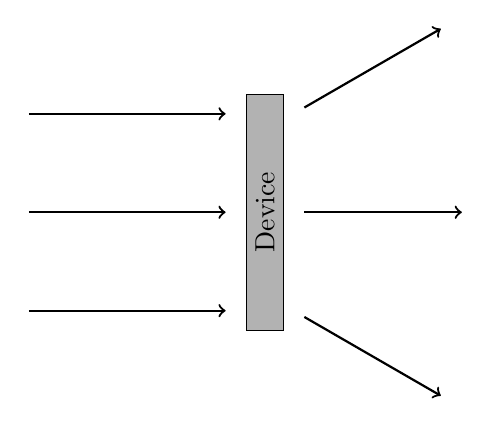
\begin{tikzpicture}
        %% device
        \node[draw,fill=white!70!black,minimum width=3cm,rotate=90] at (0,0) {Device};
        %% rays
        \foreach \x in {1.25,0,-1.25} \draw[thick,->] (-3,\x) -- (-0.5,\x);
        \foreach \x/\y in {+1.33/30,0/0,-1.33/330} \draw[thick,->] (0.5,\x) -- ++(\y:2);
    \end{tikzpicture}
    \end{center}
    The device could be a:
    \begin{choices}
        \wrongchoice{convex glass lens}
        \wrongchoice{rectangular glass block}
        \wrongchoice{plane mirror}
      \correctchoice{concave glass lens}
    \end{choices}
\end{question}
}

\element{nysed}{
\begin{question}{June2000-Q94}
    A person is standing in front of a diverging (convex) mirror.
    What type of image does the mirror form of the person?
    \begin{choices}
      \correctchoice{erect, virtual, and smaller than the person}
        \wrongchoice{erect, virtual, and the same size as the person}
        \wrongchoice{erect, real, and smaller than the person}
        \wrongchoice{erect, real, and the same size as the person}
    \end{choices}
\end{question}
}

\element{nysed}{
\begin{question}{June2000-Q95}
    Which graph best represents the relationship between image size ($S_i$) and image distance ($d_i$) for real images formed by a converging lens?
    A person is standing in front of a diverging (convex) mirror.
    What type of image does the mirror form of the person?
    \begin{multicols}{2}
    \begin{choices}
        \AMCboxDimensions{down=-2.5em}
        \wrongchoice{
            \begin{tikzpicture}
                \begin{axis}[
                    axis y line=left,
                    axis x line=bottom,
                    axis line style={->},
                    xlabel={$d_i$},
                    xtick=\empty,
                    ylabel={$S_i$},
                    ytick=\empty,
                    y label style={rotate=-90},
                    xmin=0,xmax=11,
                    ymin=0,ymax=11,
                    width=\columnwidth,
                    very thin,
                ]
                \addplot[line width=1pt,domain=0:10]{x};
                \end{axis}
            \end{tikzpicture}
        }
        \correctchoice{
            \begin{tikzpicture}
                \begin{axis}[
                    axis y line=left,
                    axis x line=bottom,
                    axis line style={->},
                    xlabel={$d_i$},
                    xtick=\empty,
                    ylabel={$S_i$},
                    ytick=\empty,
                    y label style={rotate=-90},
                    xmin=0,xmax=11,
                    ymin=0,ymax=11,
                    width=\columnwidth,
                    very thin,
                ]
                \addplot[line width=1pt,domain=0:5]{10-2*x};
                \addplot[line width=1pt,domain=5:10]{2*(x-5)};
                \end{axis}
            \end{tikzpicture}
        }
        \wrongchoice{
            \begin{tikzpicture}
                \begin{axis}[
                    axis y line=left,
                    axis x line=bottom,
                    axis line style={->},
                    xlabel={$d_i$},
                    xtick=\empty,
                    ylabel={$S_i$},
                    ytick=\empty,
                    y label style={rotate=-90},
                    xmin=0,xmax=11,
                    ymin=0,ymax=11,
                    width=\columnwidth,
                    very thin,
                ]
                \addplot[line width=1pt,domain=0:10]{0.1*x*x};
                \end{axis}
            \end{tikzpicture}
        }
        \wrongchoice{
            \begin{tikzpicture}
                \begin{axis}[
                    axis y line=left,
                    axis x line=bottom,
                    axis line style={->},
                    xlabel={$d_i$},
                    xtick=\empty,
                    ylabel={$S_i$},
                    ytick=\empty,
                    y label style={rotate=-90},
                    xmin=0,xmax=11,
                    ymin=0,ymax=11,
                    width=\columnwidth,
                    very thin,
                ]
                \addplot[line width=1pt,domain=0:10]{8};
                \end{axis}
            \end{tikzpicture}
        }
    \end{choices}
    \end{multicols}
\end{question}
}


%% Section June1999
%%--------------------
\element{nysed}{
\begin{question}{June1999-Q86}
    A lens produces a real image by causing light rays from a common point to:
    \begin{choices}
      \correctchoice{converge and intersect at a point.}
        \wrongchoice{disperse into component wavelengths.}
        \wrongchoice{reflect constructively.}
        \wrongchoice{diverge and appear to come from a point.}
    \end{choices}
\end{question}
}

\element{nysed}{
\begin{question}{June1999-Q87}
    The graph below shows the relationship between a mirror's object distance ($d_o$) and image distance ($d_i$).
    \begin{center}
    \begin{tikzpicture}
        \begin{axis}[
            axis y line=left,
            axis x line=middle,
            x axis line style={->},
            y axis line style={<-},
            xlabel={$d_o$},
            x unit=\si{\centi\meter},
            xtick={5,10,15,20},
            xticklabel style={yshift=0.5ex,anchor=south},
            xlabel style={yshift=-0.5ex,anchor=north east},
            ylabel={$d_i$},
            y unit=\si{\centi\meter},
            ytick={-20,-10,0,10,20},
            minor y tick num=1,
            xmin=0,xmax=21,
            ymin=-21,ymax=20,
            width=1.000\columnwidth,
            height=0.618\columnwidth,
            very thin,
        ]
        \addplot[line width=1pt,domain=0:20]{-x};
        \end{axis}
    \end{tikzpicture}
    \end{center}
    From which type of mirror were the data collected?
    \begin{multicols}{2}
    \begin{choices}
        \wrongchoice{concave}
        \wrongchoice{convex}
        \wrongchoice{parabolic}
      \correctchoice{plane}
    \end{choices}
    \end{multicols}
\end{question}
}

\element{nysed}{
\begin{question}{June1999-Q88}
    The diagram below shows a ray of light traveling parallel to the principal axis of a concave spherical mirror.
    Point $F$ is the principal focus and point $C$ is the center of curvature.
    \begin{center}
    \begin{tikzpicture}
        %% Mirror and  Ray
        \draw[thick] (-45:2cm) arc (-45:45:2cm) node[anchor=south] {Mirror};
        \draw [->] (-1,1) -- (1,1);
        %% Axis and Labels
        \draw (2,0) -- (-3,0) node[anchor=east] {Principal Axis};
        %% options
        \foreach \x/\y in {0/C,1/F,1.5/A,-2.0/D}
            \fill (\x,0) circle (1.5pt) node[anchor=north] {$\y$};
    \end{tikzpicture}
    \end{center}
    After striking the mirror,
        the ray of light will be reflected through point:
    \begin{multicols}{4}
    \begin{choices}[o]
        \wrongchoice{$A$}
      \correctchoice{$F$}
        \wrongchoice{$C$}
        \wrongchoice{$D$}
    \end{choices}
    \end{multicols}
\end{question}
}

%% NOTE: Finish tikz newcommand
\newcommand{\JuneNineNineQEightyNine}{
\begin{tikzpicture}
    %% mirror
    \draw[thick] (-45:2cm) arc(-45:45:2cm) node[anchor=west] {Mirror};
    \draw [->] (-1,1) -- (1,1);
    \draw (2,0) -- (-3,0) node[anchor=east] {Principal Axis};
    %% options
    \foreach \x/\y in {0/C,1/F,1.5/A,-2.0/D}
        \fill (\x,0) circle (1.5pt) node[anchor=north] {$\y$};
\end{tikzpicture}
}

\element{nysed}{
\begin{question}{June1999-Q89}
    A candle \SI{0.10}{\meter} tall is placed \SI{0.30}{\meter} from a thin converging lens.
    The crown glass lens has a focal length, $f$, of \SI{0.20}{\meter}.
    \begin{center}
        \JuneNineNineQEightyNine
        \includegraphics[keepaspectratio,scale=0.9]{June1999-Q89}
    \end{center}
    What is the distance from the lens to the candle's image?
    \begin{multicols}{2}
    \begin{choices}
        \wrongchoice{\SI{0.10}{\meter}}
        \wrongchoice{\SI{0.30}{\meter}}
        \wrongchoice{\SI{0.40}{\meter}}
      \correctchoice{\SI{0.60}{\meter}}
    \end{choices}
    \end{multicols}
\end{question}
}

\element{nysed}{
\begin{question}{June1999-Q90}
    A candle \SI{0.10}{\meter} tall is placed \SI{0.30}{\meter} from a thin converging lens.
    The crown glass lens has a focal length, $f$, of \SI{0.20}{\meter}.
    \begin{center}
        \JuneNineNineQEightyNine
        %\includegraphics[keepaspectratio,scale=0.9]{June1999-Q89}
    \end{center}
    Changing the lens material from crown glass to flint glass would cause the focal length to:
    \begin{multicols}{2}
    \begin{choices}
      \correctchoice{decrease}
        \wrongchoice{increase}
        \wrongchoice{remain the same}
    \end{choices}
    \end{multicols}
\end{question}
}

\element{nysed}{
\begin{question}{June1999-Q91}
    What type of images can be projected onto a screen?
    \begin{choices}
      \correctchoice{real images, only}
        \wrongchoice{virtual images, only}
        \wrongchoice{both real images and virtual images}
        \wrongchoice{neither real images nor virtual images}
    \end{choices}
\end{question}
}

\element{nysed}{
\begin{question}{June1999-Q92}
    An object is located \SI{0.40}{\meter} in front of a diverging lens having a focal length of \SI{-0.20}{\meter}.
    Compared to the object, the image formed by the lens is:
    \begin{choices}
        \wrongchoice{smaller, inverted, and real}
        \wrongchoice{larger, inverted and real}
      \correctchoice{smaller, erect and virtual}
        \wrongchoice{larger, erect, and virtual}
    \end{choices}
\end{question}
}

\element{nysed}{
\begin{question}{June1999-Q93}
    In the diagram below, a candle is located at point $P$ in front of a concave spherical mirror.
    Point $F$ is the principal focus of the mirror,
        and point $C$ is the center of curvature.
    \begin{center}
    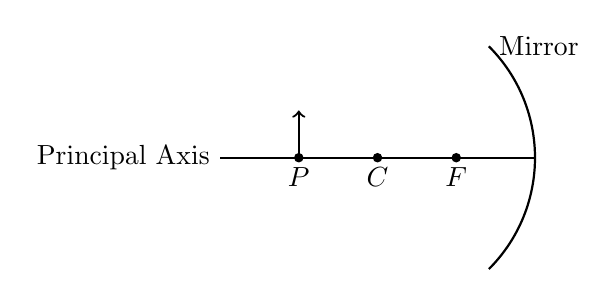
\begin{tikzpicture}
        %% Mirror
        \draw[thick] (-45:2cm) arc (-45:45:2cm)
            node[anchor=west] {Mirror};
            %node[pos=0.5,anchor=south west] {Concave}
            %node[pos=0.5,anchor=north west] {Mirror};
        %% Principal Axis
        \draw [thick] (2,0) -- (-2,0)
            node[anchor=east] {Principal Axis};
        \draw[fill] (0,0) circle (1.5pt)
            node[anchor=north] {$C$};
        \draw[fill] (1.0,0) circle (1.5pt)
            node[anchor=north] {$F$};
        %% Object
        \draw[fill] (-1.0,0) circle (1.5pt)
            node[anchor=north] {$P$};
        \draw[thick,->] (-1.0,0) -- (-1.0,0.6);
    \end{tikzpicture}
    \end{center}
    As the candle is moved from point $P$ toward point $C$, the size of its image:
    \begin{choices}
        \wrongchoice{decreases}
      \correctchoice{increases}
        \wrongchoice{remain the same}
    \end{choices}
\end{question}
}

\element{nysed}{
\begin{question}{June1999-Q93}
    In the diagram below, a candle is located at point $P$ in front of a concave spherical mirror.
    Point $F$ is the principal focus of the mirror,
        and point $C$ is the center of curvature.
    \begin{center}
    \begin{tikzpicture}
        %% NOTE: finish mirror ray diagram
    \end{tikzpicture}
    \end{center}
    As the candle is moved from point $P$ toward point $C$,
        the size of the image:
    \begin{choices}
        \wrongchoice{decrease}
      \correctchoice{increase}
        \wrongchoice{remain the same}
    \end{choices}
\end{question}
}

\element{nysed}{
\begin{question}{June1999-Q94}
    An object \SI{0.15}{\meter} tall placed \SI{0.25}{\meter} in front of a concave mirror produced an image \SI{0.20}{\meter} tall.
    The image distance is approximately:
    \begin{multicols}{2}
    \begin{choices}
        \wrongchoice{\SI{0.12}{\meter}}
        \wrongchoice{\SI{0.19}{\meter}}
      \correctchoice{\SI{0.33}{\meter}}
        \wrongchoice{\SI{0.45}{\meter}}
    \end{choices}
    \end{multicols}
\end{question}
}

\element{nysed}{
\begin{question}{June1999-Q95}
    Spherical aberration is a defect associated with:
    \begin{choices}
        \wrongchoice{lenses, only}
        \wrongchoice{plane mirrors}
        \wrongchoice{spherical mirrors, only}
      \correctchoice{lenses and spherical mirrors}
    \end{choices}
\end{question}
}


%% Section June1998
%%--------------------
\element{nysed}{
\begin{question}{June1998-Q86}
    When a \SI{0.020}{\meter} tall object is placed \SI{0.15}{\meter} in front of a converging mirror,
        the object's image appears \SI{0.30}{\meter} in front of the mirror.
    The focal length of the mirror is:
    \begin{multicols}{2}
    \begin{choices}
        \wrongchoice{\SI{0.45}{\meter}}
      \correctchoice{\SI{0.1}{\meter}}
        \wrongchoice{\SI{-0.10}{\meter}}
        \wrongchoice{\SI{-0.15}{\meter}}
    \end{choices}
    \end{multicols}
\end{question}
}

\element{nysed}{
\begin{question}{June1998-Q87}
    When a \SI{0.020}{\meter} tall object is placed \SI{0.15}{\meter} in front of a converging mirror,
        the object's image appears \SI{0.30}{\meter} in front of the mirror.
    How tall is the image?
    \begin{multicols}{2}
    \begin{choices}
        \wrongchoice{\SI{0.010}{\meter}}
        \wrongchoice{\SI{0.020}{\meter}}
        \wrongchoice{\SI{0.030}{\meter}}
      \correctchoice{\SI{0.040}{\meter}}
    \end{choices}
    \end{multicols}
\end{question}
}

\element{nysed}{
\begin{question}{June1998-Q89}
    The diagram below shows a light ray parallel to the principal axis of a spherical convex (diverging) mirror.
    Point $F$ is the virtual focal point of the mirror and $C$ is the center of curvature.
    \begin{center}
    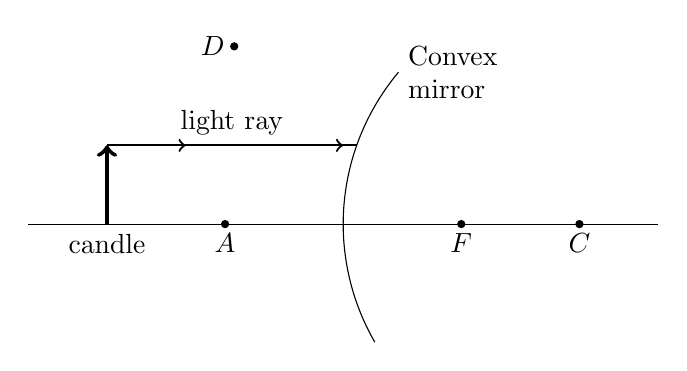
\begin{tikzpicture}
        %% principal axis
        \draw (-4,0) -- (4,0);
        %% candle
        \draw[ultra thick,->] (-3,0) -- (-3,1);
        \node[anchor=north] at (-3,0) {candle};
        %% mirror
        \draw (0,0) arc(180:140:3) node[anchor=west,text width=4em] {Convex mirror};
        \draw (0,0) arc(180:210:3);
        %% ray
        \draw[thick] (-3,1) -- ({3*(1-sqrt(1-1/9))},1) node[pos=0.5,anchor=south] {light ray};
        \draw[thick,->] (-0.5,1) -- ++(0:0.5);
        \draw[thick,->] (-2.5,1) -- ++(0:0.5);
        %\draw[thick,->] ({3*(1-sqrt(1-1/9))},1) -- ++(141.05:2);
        %% points A, F, C
        \fill (-1.5,0) circle (1.5pt) node[anchor=north] {$A$};
        \fill (+1.5,0) circle (1.5pt) node[anchor=north] {$F$};
        \fill (+3,0) circle (1.5pt) node[anchor=north] {$C$};
        \fill ({3*(1-sqrt(1-1/9))},1) ++(141.05:2) circle (1.5pt) node[anchor=east] {$D$};
    \end{tikzpicture}
    \end{center}
    After the light ray is reflected, it will pass through:
    \begin{multicols}{4}
    \begin{choices}[o]
        \wrongchoice{$A$}
        \wrongchoice{$F$}
        \wrongchoice{$C$}
      \correctchoice{$D$}
    \end{choices}
    \end{multicols}
\end{question}
}

\newcommand{\nysedJuneNineteenNineyNineQNinety}{
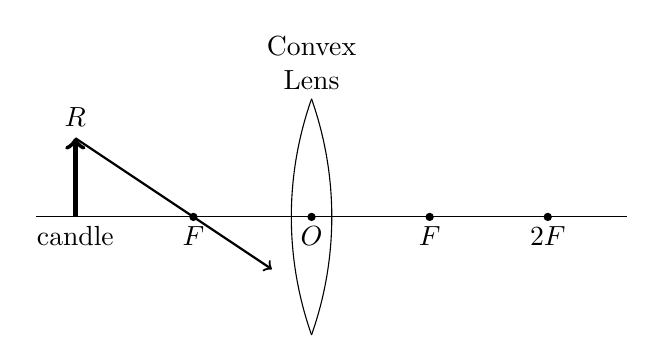
\begin{tikzpicture}
    %% principal axis
    \draw (-3.5,0) -- (4,0);
    %% Candle
    \draw[ultra thick,->] (-3,0) -- (-3,1) node[anchor=south] {$R$};
    \node[anchor=north] at (-3,0) {candle};
    \draw[thick,->] (-3,1) -- ++(326.31:3);
    %% convex lens
    \foreach \x in {-19.47,19.47} {
        \draw (-0.257,0) arc(180:{180+\x}:4.5);
        \draw (+0.257,0) arc(0:{0+\x}:4.5);
    }
    \node[anchor=south,text width=4em,text centered] at (0,1.5) {Convex Lens};
    %% labels
    \foreach \x/\y in {-1.5/F,0/O,1.5/F,3/2F}
        \fill (\x,0) circle (1.5pt) node[anchor=north] {$\y$};
\end{tikzpicture}
}

\element{nysed}{
\begin{question}{June1998-Q90}
    A convex lens having optical center $O$ and principal focus $F$ is used to produce an image of a candle.
    Ray $RF$ is shown.
    \begin{center}
        \nysedJuneNineteenNineyNineQNinety
    \end{center}
    The lens is being used to produce an image of the candle that is:
    \begin{choices}
        \wrongchoice{virtual and erect}
        \wrongchoice{virtual and inverted}
        \wrongchoice{real and erect}
      \correctchoice{real and inverted}
    \end{choices}
\end{question}
}

\element{nysed}{
\begin{question}{June1998-Q91}
    A convex lens having optical center $O$ and principal focus $F$ is used to produce an image of a candle.
    Ray $RF$ is shown.
    \begin{center}
        \nysedJuneNineteenNineyNineQNinety
    \end{center}
    When ray $RF$ reaches the lens, the ray will:
    \begin{choices}
        \wrongchoice{reflect back through point $R$}
        \wrongchoice{polarize and travel perpendicular to the principal axis}
        \wrongchoice{refract and pass through point $2F$}
      \correctchoice{refract and emerge parallel to the principal axis}
    \end{choices}
\end{question}
}
    
\element{nysed}{
\begin{question}{June1998-Q92}
    A convex lens having optical center $O$ and principal focus $F$ is used to produce an image of a candle.
    Ray $RF$ is shown.
    \begin{center}
        \nysedJuneNineteenNineyNineQNinety
    \end{center}
    As the candle is moved toward the left,
        the size of its image will:
    \begin{choices}
      \correctchoice{decrease}
        \wrongchoice{increase}
        \wrongchoice{remain the same}
    \end{choices}
\end{question}
}

\element{nysed}{
\begin{question}{June1998-Q93}
    A \SI{2.0}{\meter} tall student is able to view his entire body at once using a plane marrow.
    The minimum length of the morrow is
    \begin{multicols}{2}
    \begin{choices}
      \correctchoice{\SI{1.0}{\meter}}
        \wrongchoice{\SI{0.50}{\meter}}
        \wrongchoice{\SI{1.5}{\meter}}
        \wrongchoice{\SI{2.5}{\meter}}
    \end{choices}
    \end{multicols}
\end{question}
}

\element{nysed}{
\begin{question}{June1998-Q94}
    The filament in an automobile headlight radiates light that is reflected from a concave (converging) mirror.
    The reflected rays form a parallel beam of light because the filament is placed:
    \begin{choices}
        \wrongchoice{between the mirror and the principal focus.}
      \correctchoice{at the mirror's principal focus.}
        \wrongchoice{at the mirror's center of curvature.}
        \wrongchoice{beyond the mirror's center of curvature.}
    \end{choices}
\end{question}
}

\element{nysed}{
\begin{question}{June1998-Q95}
    Which phenomenon may cause a concave mirror to form fuzzy, out of focus images?
    \begin{choices}
      \correctchoice{spherical aberration}
        \wrongchoice{chromatic aberration}
        \wrongchoice{dispersion}
        \wrongchoice{refraction}
    \end{choices}
\end{question}
}


%% Section June1997
%%--------------------
\element{nysed}{
\begin{question}{June1997-Q86}
    In the diagram below,
        a source produces a light ray that is reflected from a plane mirror.
    \begin{center}
    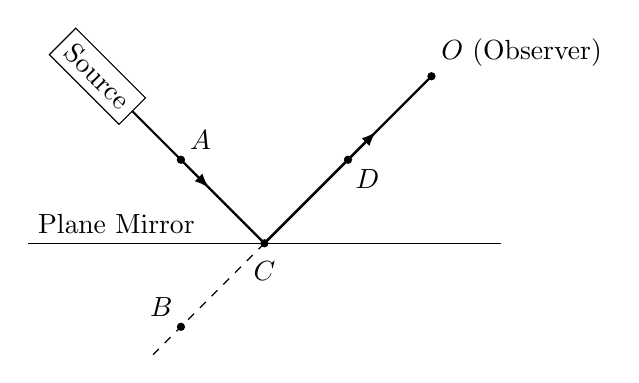
\begin{tikzpicture}
        %% plane mirror
        \draw (-3,0) -- (3,0);
        \node[anchor=south west] at (-3,0) {Plane Mirror};
        %% source
        \node[draw,anchor=center,rotate=-45] (S) at (135:3) {Source};
        \draw[thick] (S.east) -- (0,0) -- (45:3);
        \draw[dashed] (0,0) -- (225:2);
        %% ray arrows
        \draw[thick,-latex] (0,0) -- (45:2);
        \draw[thick,-latex] (0,0) -- (135:1.5) -- ++(315:0.5);
        %% observer
        \fill (45:3) circle (1.5pt) node[anchor=south west] {$O$ (Observer)};
        %% options
        \foreach \x/\y/\z in  {135/1.5/A,45/1.5/D,0/0/C,225/1.5/B}
            \fill (\x:\y) circle (1.5pt) node[anchor=center,shift={({\x-90}:1em)}] {$\z$};
    \end{tikzpicture}
    \end{center}
    To an observer at point $O$,
        the light appears to originate from point:
    \begin{multicols}{4}
    \begin{choices}[o]
        \wrongchoice{$A$}
      \correctchoice{$B$}
        \wrongchoice{$C$}
        \wrongchoice{$D$}
    \end{choices}
    \end{multicols}
\end{question}
}

\element{nysed}{
\begin{question}{June1997-Q87}
    A spherical mirror that forms only virtual images has a radius of curvature of \SI{0.50}{\meter}.
    The focal length of this mirror is:
    \begin{multicols}{2}
    \begin{choices}
      \correctchoice{\SI{-0.25}{\meter}}
        \wrongchoice{\SI[retain-explicit-plus]{+0.25}{\meter}}
        \wrongchoice{\SI{-0.50}{\meter}}
        \wrongchoice{\SI[retain-explicit-plus]{+0.50}{\meter}}
    \end{choices}
    \end{multicols}
\end{question}
}

\element{nysed}{
\begin{question}{June1997-Q88}
    A spherical concave mirror is used in the back of a car headlight.
    Where must the bulb of the headlight be located to produce a parallel beam of reflected light?
    \begin{choices}
        \wrongchoice{between the principal focus and the mirror}
        \wrongchoice{beyond the center of curvature of the mirror}
      \correctchoice{at the principal focus of the mirror}
        \wrongchoice{at the center of curvature of the mirror}
    \end{choices}
\end{question}
}

\newcommand{\nysedJuneNineteenNinetySevenQEightyNine}{
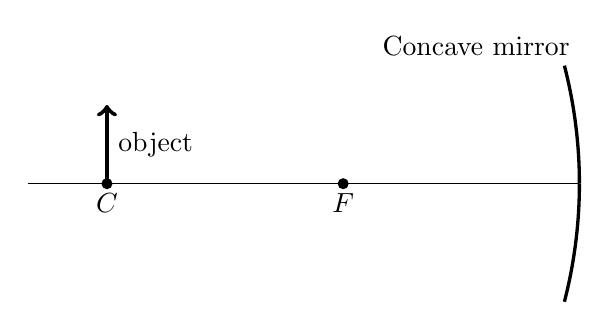
\begin{tikzpicture}
    %% principal axis
    \draw (-7,0) -- (0,0);
    %% candle
    \draw[ultra thick,->] (-6,0) -- (-6,1) node[pos=0.5,anchor=west] {object};
    %% mirror
    \node[anchor=south east] at (0,1.5) {Concave mirror};
    \draw[very thick] (0,0) arc(0:+14.47:6);
    \draw[very thick] (0,0) arc(0:-14.47:6);
    %% points C, F
    \foreach \x/\y in {-3/F,-6/C}
        \fill (\x,0) circle (2pt) node[anchor=north] {$\y$};
\end{tikzpicture}
}

\element{nysed}{
\begin{question}{June1997-Q89}
    An object is located at the center of curvature $C$ of a concave spherical mirror with principal focus $F$.
    The focal length of the mirror is \SI{0.10}{\meter}.
    \begin{center}
        \nysedJuneNineteenNinetySevenQEightyNine
    \end{center}
    At what distance from the mirror is the image located?
    \begin{multicols}{2}
    \begin{choices}
        \wrongchoice{\SI{0.10}{\meter}}
      \correctchoice{\SI{0.20}{\meter}}
        \wrongchoice{\SI{0.30}{\meter}}
        \wrongchoice{\SI{0.40}{\meter}}
    \end{choices}
    \end{multicols}
\end{question}
}

\element{nysed}{
\begin{question}{June1997-Q90}
    An object is located at the center of curvature $C$ of a concave spherical mirror with principal focus $F$.
    The focal length of the mirror is \SI{0.10}{\meter}.
    \begin{center}
        \nysedJuneNineteenNinetySevenQEightyNine
    \end{center}
    At what distance from the mirror could the object be placed to produce a virtual image of the object?
    \begin{multicols}{2}
    \begin{choices}
      \correctchoice{\SI{0.05}{\meter}}
        \wrongchoice{\SI{0.10}{\meter}}
        \wrongchoice{\SI{0.30}{\meter}}
        \wrongchoice{\SI{0.50}{\meter}}
    \end{choices}
    \end{multicols}
\end{question}
}

\element{nysed}{
\begin{question}{June1997-Q91}
    An object is located at the center of curvature $C$ of a concave spherical mirror with principal focus $F$.
    The focal length of the mirror is \SI{0.10}{\meter}.
    \begin{center}
        \nysedJuneNineteenNinetySevenQEightyNine
    \end{center}
    As the object is moved from point $C$ toward point $F$,
        the size of its image:
    \begin{multicols}{2}
    \begin{choices}
        \wrongchoice{decreases}
      \correctchoice{increases}
        \wrongchoice{remains the same}
    \end{choices}
    \end{multicols}
\end{question}
}

\element{nysed}{
\begin{question}{June1997-Q92}
    A crown glass converging lens has a focal length of \SI{0.10}{\meter}.
    Which cross-sectional diagram best represents this lens?
    \begin{multicols}{4}
    \begin{choices}
        \def\r{4}
        \AMCboxDimensions{down=-1.4cm}
        \wrongchoice{
            \begin{tikzpicture}
                \draw[fill=white!90!black] (0.50,-1.5) -- (0,-1.5) -- (0,1.5) -- (0.5,1.5) arc({180-asin(1.5/\r)}:{180+asin(1.5/\r)}:\r) -- cycle;
            \end{tikzpicture}
        }
        \wrongchoice{
            \begin{tikzpicture}
                %\draw[fill=white!90!black] (0.50,-1.5) -- (-0.50,-1.5) arc({-asin(1.5/\r)}:{asin(1.5/\r)}:\r) -- (0.50,1.5) arc({180-asin(1.5/\r)}:{180+asin(1.5/\r)}:\r) -- cycle;
                \draw[fill=white!90!black] (0.33,-1.5) -- (-0.33,-1.5) arc({-asin(0.75*1.5/\r)}:{asin(0.75*1.5/\r)}:{1.33*\r}) -- (0.33,1.5) arc({180-asin(0.75*1.5/\r)}:{180+asin(0.75*1.5/\r)}:{1.33*\r}) -- cycle;
            \end{tikzpicture}
        }
        \wrongchoice{
            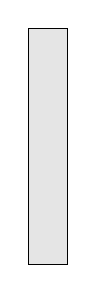
\begin{tikzpicture}
                \draw[fill=white!90!black] (0.25,-1.5) -- (0,-1.5) -- (0,1.5) -- (0.5,1.5) -- (0.5,-1.5) -- cycle;
            \end{tikzpicture}
        }
        \correctchoice{
            \begin{tikzpicture}
                \draw[fill=white!90!black] (0,-1.5) -- (0,1.5) arc({asin(1.5*1.5/\r)}:{-asin(1.5*1.5/\r)}:{0.66*\r}) -- cycle;
            \end{tikzpicture}
        }
    \end{choices}
    \end{multicols}
\end{question}
}

\element{nysed}{
\begin{question}{June1997-Q93}
    A crown glass converging lens has a focal length of \SI{0.10}{\meter}.
    An object is placed \SI{0.30}{\meter} from the lens.
    How far from the lens will an image of the object be formed?
    \begin{multicols}{2}
    \begin{choices}
        \wrongchoice{\SI{0.30}{\meter}}
        \wrongchoice{\SI{0.20}{\meter}}
      \correctchoice{\SI{0.15}{\meter}}
        \wrongchoice{\SI{0.10}{\meter}}
    \end{choices}
    \end{multicols}
\end{question}
}

\element{nysed}{
\begin{question}{June1997-Q94}
    An object \SI{0.800}{\meter} high is placed \SI{0.20}{\meter} from a converging (convex) lens.
    If the distance of the image from the lens is \SI{0.40}{\meter}, the height of the image is
    \begin{multicols}{2}
    \begin{choices}
        \wrongchoice{\SI{0.010}{\meter}}
      \correctchoice{\SI{0.040}{\meter}}
        \wrongchoice{\SI{0.080}{\meter}}
        \wrongchoice{\SI{0.16}{\meter}}
    \end{choices}
    \end{multicols}
\end{question}
}

\element{nysed}{
\begin{question}{June1997-Q95}
    A diverging (concave) lens can form images that are:
    \begin{choices}
      \correctchoice{virtual, only}
        \wrongchoice{inverted, only}
        \wrongchoice{either virtual or real}
        \wrongchoice{either inverted or erect}
    \end{choices}
\end{question}
}


%% Section June1996
%%--------------------
\element{nysed}{
\begin{question}{June1996-Q86}
    A plane mirror will form an image that is:
    \begin{choices}
      \correctchoice{virtual and erect}
        \wrongchoice{real and inverted}
        \wrongchoice{virtual and inverted}
        \wrongchoice{real and erect}
    \end{choices}
\end{question}
}

\element{nysed}{
\begin{question}{June1996-Q87}
    Which graph best represents the relationship between image distance ($d_i$) and object distance ($d_o$) for a plane mirror?
    \begin{multicols}{2}
    \begin{choices}
        \AMCboxDimensions{down=-2.5em}
        \correctchoice{
            \begin{tikzpicture}
                \begin{axis}[
                    axis y line=left,
                    axis x line=bottom,
                    axis line style={->},
                    xlabel={$d_i$},
                    xtick=\empty,
                    ylabel={$d_o$},
                    ytick=\empty,
                    y label style={rotate=-90},
                    xmin=0,xmax=11,
                    ymin=0,ymax=11,
                    width=\columnwidth,
                    very thin,
                ]
                \addplot[line width=1pt,domain=0:10]{x};
                \end{axis}
            \end{tikzpicture}
        }
        \wrongchoice{
            \begin{tikzpicture}
                \begin{axis}[
                    axis y line=left,
                    axis x line=bottom,
                    axis line style={->},
                    xlabel={$d_i$},
                    xtick=\empty,
                    ylabel={$d_o$},
                    ytick=\empty,
                    y label style={rotate=-90},
                    xmin=0,xmax=11,
                    ymin=0,ymax=11,
                    width=\columnwidth,
                    very thin,
                ]
                \addplot[line width=1pt,domain=0:10]{0.1*x*x};
                \end{axis}
            \end{tikzpicture}
        }
        \wrongchoice{
            \begin{tikzpicture}
                \begin{axis}[
                    axis y line=left,
                    axis x line=bottom,
                    axis line style={->},
                    xlabel={$d_i$},
                    xtick=\empty,
                    ylabel={$d_o$},
                    ytick=\empty,
                    y label style={rotate=-90},
                    xmin=0,xmax=11,
                    ymin=0,ymax=11,
                    width=\columnwidth,
                    very thin,
                ]
                \addplot[line width=1pt,domain=0:10]{10/x};
                \end{axis}
            \end{tikzpicture}
        }
        \wrongchoice{
            \begin{tikzpicture}
                \begin{axis}[
                    axis y line=left,
                    axis x line=bottom,
                    axis line style={->},
                    xlabel={$d_i$},
                    xtick=\empty,
                    ylabel={$d_o$},
                    ytick=\empty,
                    y label style={rotate=-90},
                    xmin=0,xmax=11,
                    ymin=0,ymax=11,
                    width=\columnwidth,
                    very thin,
                ]
                \addplot[line width=1pt,domain=0:10]{8};
                \end{axis}
            \end{tikzpicture}
        }
    \end{choices}
    \end{multicols}
\end{question}
}

\element{nysed}{
\begin{question}{June1996-Q88}
    Which lens defect is correctly paired with its cause?
    \begin{choices}
      \correctchoice{chromatic aberration, caused by refraction}
        \wrongchoice{real and inverted}
        \wrongchoice{virtual and inverted}
        \wrongchoice{real and erect}
    \end{choices}
\end{question}
}

\newcommand{\nysedJuneNineteenNinetySixQEightyNine}{
\begin{tikzpicture}[scale=0.9]
    \draw (8.5,0) -- (0,0);
    %% mirror
    \node[anchor=south west] at (0,1.5) {mirror};
    \draw[very thick] (0,0) arc(180:{180-asin(1.5/8)}:8);
    \draw[very thick] (0,0) arc(180:{180+asin(1.5/8)}:8);
    %% points A, F, C
    \foreach \x/\y in {2/A,4/F,8/C}
        \fill (\x,0) circle (2pt) node[anchor=north] {$\y$};
\end{tikzpicture}
}

\element{nysed}{
\begin{question}{June1996-Q89}
<<<<<<< HEAD
    The diagram shows a concave (converging) spherical mirror having principal focus $F$ and center of curvatur $C$.
=======
    The diagram shows a concave (converging) spherical mirror having principal focus $F$ and center of curvature $C$.
>>>>>>> develop
    Point $A$ lies on the principal axis.
    \begin{center}
        \nysedJuneNineteenNinetySixQEightyNine
    \end{center}
    When an object is placed at point $A$,
        its image is observed:
    \begin{choices}
        \wrongchoice{at $F$}
        \wrongchoice{between $F$ and $C$}
        \wrongchoice{to the left of $C$}
      \correctchoice{to the left of the mirror}
    \end{choices}
\end{question}
}

\element{nysed}{
\begin{question}{June1996-Q90}
<<<<<<< HEAD
    The diagram shows a concave (converging) spherical mirror having principal focus $F$ and center of curvatur $C$.
=======
    The diagram shows a concave (converging) spherical mirror having principal focus $F$ and center of curvature $C$.
>>>>>>> develop
    Point $A$ lies on the principal axis.
    \begin{center}
        \nysedJuneNineteenNinetySixQEightyNine
    \end{center}
    If an object is located at point $A$,
        its image is:
    \begin{choices}
        \wrongchoice{virtual and inverted}
      \correctchoice{virtual and erect}
        \wrongchoice{real and inverted}
        \wrongchoice{read and erect}
    \end{choices}
\end{question}
}

\element{nysed}{
\begin{question}{June1996-Q91}
    Which phenomenon allows a lens to focus light?
    \begin{multicols}{2}
    \begin{choices}
        \wrongchoice{diffraction}
      \correctchoice{refraction}
        \wrongchoice{interference}
        \wrongchoice{polarization}
    \end{choices}
    \end{multicols}
\end{question}
}

\element{nysed}{
\begin{question}{June1996-Q92}
    The diagram below represents an object placed two focal lengths from a converging lens.
    \begin{center}
    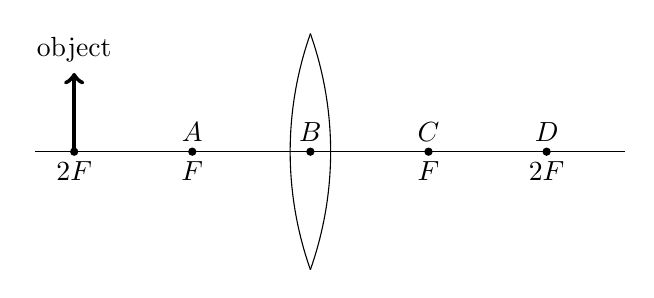
\begin{tikzpicture}
        %% principal axis
        \draw (-3.5,0) -- (4,0);
        %% Candle
        \draw[ultra thick,->] (-3,0) -- (-3,1) node[anchor=south] {object};
        %% convex lens
        \foreach \x in {-19.47,19.47} {
            \draw (-0.257,0) arc(180:{180+\x}:4.5);
            \draw (+0.257,0) arc(0:{0+\x}:4.5);
        }
        %% labels
        \foreach \x/\y in {-3/2F,-1.5/F,1.5/F,3/2F}
            \fill (\x,0) circle (1.5pt) node[anchor=north] {$\y$};
        %% options
        \fill (0,0) circle (1.5pt);
        \foreach \x/\y in {-1.5/A,0/B,1.5/C,3/D}
            \node[anchor=south] at (\x,0) {$\y$};
    \end{tikzpicture}
    \end{center}
    At which point will the image be located?
    \begin{multicols}{4}
    \begin{choices}
        \wrongchoice{$A$}
        \wrongchoice{$B$}
        \wrongchoice{$C$}
      \correctchoice{$D$}
    \end{choices}
    \end{multicols}
\end{question}
}

\element{nysed}{
\begin{question}{June1996-Q93}
    An image that is \SI{1.0e-2}{\meter} tall is formed on a screen behind a converging lens when an object \SI{2.0}{\meter} tall is placed \SI{8.0}{\meter} in front of the lens.
    What is the distance from the lens to the screen?
    \begin{multicols}{2}
    \begin{choices}
        \wrongchoice{\SI{2.5e-3}{\meter}}
        \wrongchoice{\SI{2.5e-1}{\meter}}
        \wrongchoice{\SI{4.0e-2}{\meter}}
      \correctchoice{\SI{4.0e-1}{\meter}}
    \end{choices}
    \end{multicols}
\end{question}
}

\element{nysed}{
\begin{question}{June1996-Q94}
    A student uses a magnifying glass to examine the crystals in a mineral specimen.
    The magnifying glass contains a:
    \begin{choices}
        \wrongchoice{convex (diverging) mirror}
      \correctchoice{convex (converging) lens}
        \wrongchoice{concave (diverging) lens}
        \wrongchoice{plane mirror}
    \end{choices}
\end{question}
}

\element{nysed}{
\begin{question}{June1996-Q95}
    The focal length of a lens is \emph{not} dependent on the:
    \begin{choices}
        \wrongchoice{material from which the lens is made}
        \wrongchoice{color of the light incident on the lens}
      \correctchoice{distance of an object from the lens}
        \wrongchoice{shape or curvature of the lens}
    \end{choices}
\end{question}
}


%% Section June1995
%%--------------------
\element{nysed}{
\begin{question}{June1995-Q86}
    A truck has the letters ``OWOW'' printed on the front of its hood.
    A person in a car driving ahead of the truck views these letters in the rear-view mirror.
    How do the letters appear?
    \begin{multicols}{2}
    \begin{choices}
        %% NOTE: TODO: Tikz rotate
      \correctchoice{WOWO}
        \wrongchoice{OWOW}
        \wrongchoice{OMOM}
        \wrongchoice{MOMO}
    \end{choices}
    \end{multicols}
\end{question}
}

\element{nysed}{
\begin{question}{June1995-Q87}
    A concave mirror has a radius of curvature of \SI{0.60}{\meter}.
    When an object is placed \SI{0.40}{\meter} from the reflecting surface,
        the image distance will be:
    \begin{multicols}{2}
    \begin{choices}
        \wrongchoice{\SI{0.10}{\meter}}
        \wrongchoice{\SI{0.20}{\meter}}
        \wrongchoice{\SI{0.83}{\meter}}
      \correctchoice{\SI{1.2}{\meter}}
    \end{choices}
    \end{multicols}
\end{question}
}

\element{nysed}{
\begin{question}{June1995-Q88}
    The diagram below shows parallel monochromatic incident light rays being reflected from a concave mirror.
    \begin{center}
    \begin{tikzpicture}
        \def\r{4}
        %% principal axis
        \draw (-7,0) -- (0,0);
        \node[anchor=north west] at (-7,0) {Principal axis};
        %% concave mirror
        \draw[very thick] (0,0) arc(0:{asin(3/\r)}:\r);
        \draw[very thick] (0,0) arc(0:{-asin(3/\r)}:\r);
        %% Rays
        \begin{scope}[decoration={markings,mark=at position 0.25 with {\arrow{latex}}}]
            \foreach \y in {-2,-1,1,2}
                \draw[thick,-latex,postaction={decorate}] (-6,\y) -- ({-\r*(1-sqrt(1-(\y/\r)^2))},\y) -- ++ ({180+2.1*asin(\y/\r)}:3.66);
        \end{scope}
    \end{tikzpicture}
    \end{center}
    Which phenomenon does the diagram illustrate?
    \begin{choices}
        \wrongchoice{chromatic aberration}
      \correctchoice{spherical aberration}
        \wrongchoice{refraction}
        \wrongchoice{dispersion}
    \end{choices}
\end{question}
}

\element{nysed}{
\begin{question}{June1995-Q89}
    Which piece of glass could be used to focus parallel rays of sunlight to a small spot of light?
    \begin{multicols}{2}
    \begin{choices}
        \AMCboxDimensions{down=-1.2cm}
        \wrongchoice{
            \begin{tikzpicture}
                \draw[dashed,white!60!black] (-1.5,-1.5) rectangle (1.5,1.5);
                \draw[thick] (-0.2,-1.25) rectangle (0.2,1.25);
            \end{tikzpicture}
        }
        %% ANS is 2
        \correctchoice{
            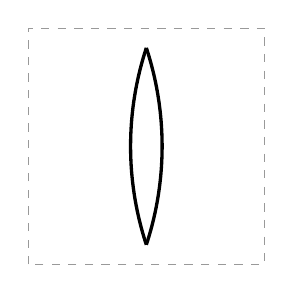
\begin{tikzpicture}
                \def\r{4}
                \draw[dashed,white!60!black] (-1.5,-1.5) rectangle (1.5,1.5);
                \draw[very thick] (0,1.25) arc({asin(1.25/\r)}:{-asin(1.25/\r)}:\r);
                \draw[very thick] (0,1.25) arc({180-asin(1.25/\r)}:{180+asin(1.25/\r)}:\r);
            \end{tikzpicture}
        }
        \wrongchoice{
            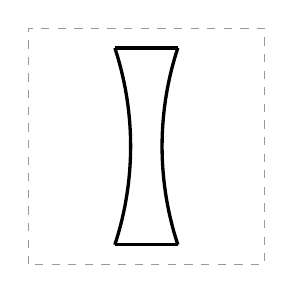
\begin{tikzpicture}
                \def\r{4}
                \draw[dashed,white!60!black] (-1.5,-1.5) rectangle (1.5,1.5);
                \draw[very thick] (-0.4,+1.25) -- (+0.4,+1.25);
                \draw[very thick] (-0.4,-1.25) -- (+0.4,-1.25);
                \draw[very thick] (-0.4,1.25) arc({asin(1.25/\r)}:{-asin(1.25/\r)}:\r);
                \draw[very thick] (+0.4,1.25) arc({180-asin(1.25/\r)}:{180+asin(1.25/\r)}:\r);
            \end{tikzpicture}
        }
        \wrongchoice{
            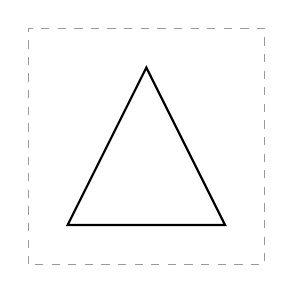
\begin{tikzpicture}
                \draw[dashed,white!60!black] (-1.5,-1.5) rectangle (1.5,1.5);
                \draw[thick] (-1,-1) -- (0,1) -- (1,-1) --cycle;
            \end{tikzpicture}
        }
    \end{choices}
    \end{multicols}
\end{question}
}

\element{nysed}{
\begin{question}{June1995-Q90}
    In the diagram below, a lamp \SI{0.4}{\meter} tall is placed \SI{0.6}{\meter} in front of a convex mirror.
    \begin{center}
    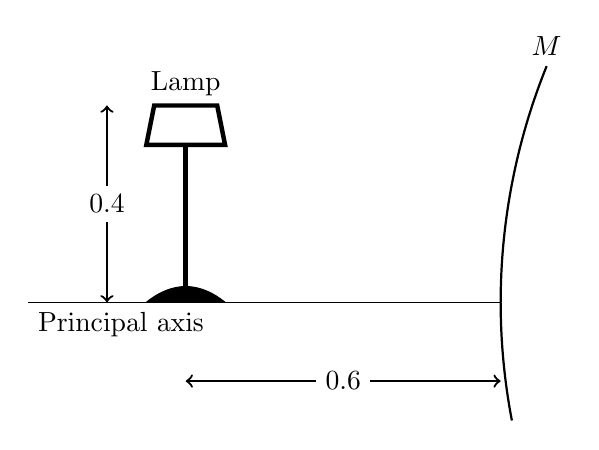
\begin{tikzpicture}
        %% principal axis
        \draw (-6,0) -- (0,0);
        \node[anchor=north west] at (-6,0) {Principal axis};
        \draw[thick] (0,0) arc (180:{180-asin(3/8)}:8) node[anchor=south] {$M$};
        \draw[thick] (0,0) arc (180:{180+asin(1.5/8)}:8);
        \draw[thick,<->] (-4,-1) -- (0,-1) node[pos=0.5,anchor=center,fill=white] {\SI{0.6}{\meter}};
        \begin{scope}[xshift=-4cm]
            %% labels
            \draw[thick,<->] (-1,0) -- (-1,2.5) node[pos=0.5,anchor=center,fill=white] {\SI{0.4}{\meter}};
            \node[anchor=south] at (0,2.5) {Lamp};
            %% lamp
            \draw[ultra thick] (-0.5,2) -- (-0.4,2.5) -- (0.4,2.5) -- (0.5,2) -- cycle;
            \draw[ultra thick] (0,0) -- (0,2);
            \draw[fill] (-0.5,0) parabola bend (0,0.2) (0.5,0) -- cycle;
        \end{scope}
    \end{tikzpicture}
    \end{center}
    Which diagram best represents an image of the lamp that could be formed by this mirror?
    \begin{multicols}{2}
    \begin{choices}
        \AMCboxDimensions{down=-1cm}
        %% NOTE: ANS is 1
        \correctchoice{
            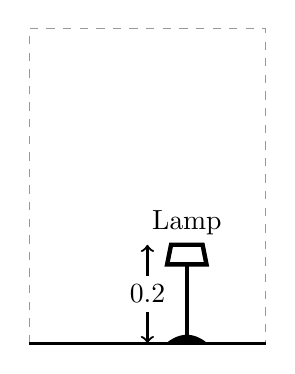
\begin{tikzpicture}
                \draw[dashed,white!60!black] (-2,0) rectangle (1,4);
                \draw[very thick] (-2,0) -- (1,0);
                \begin{scope}[scale=0.5]
                    %% labels
                    \draw[thick,<->] (-1,0) -- (-1,2.5) node[pos=0.5,anchor=center,fill=white] {\SI{0.2}{\meter}};
                    \node[anchor=south] at (0,2.5) {Lamp};
                    %% lamp
                    \draw[ultra thick] (-0.5,2) -- (-0.4,2.5) -- (0.4,2.5) -- (0.5,2) -- cycle;
                    \draw[ultra thick] (0,0) -- (0,2);
                    \draw[fill] (-0.5,0) parabola bend (0,0.2) (0.5,0) -- cycle;
                \end{scope}
            \end{tikzpicture}
        }
        \wrongchoice{
            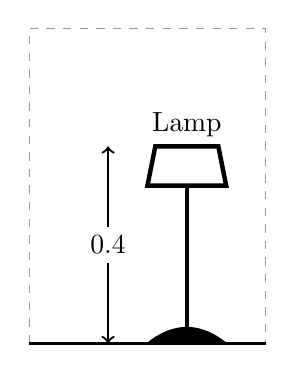
\begin{tikzpicture}
                \draw[dashed,white!60!black] (-2,0) rectangle (1,4);
                \draw[very thick] (-2,0) -- (1,0);
                \begin{scope}[scale=1.0]
                    %% labels
                    \draw[thick,<->] (-1,0) -- (-1,2.5) node[pos=0.5,anchor=center,fill=white] {\SI{0.4}{\meter}};
                    \node[anchor=south] at (0,2.5) {Lamp};
                    %% lamp
                    \draw[ultra thick] (-0.5,2) -- (-0.4,2.5) -- (0.4,2.5) -- (0.5,2) -- cycle;
                    \draw[ultra thick] (0,0) -- (0,2);
                    \draw[fill] (-0.5,0) parabola bend (0,0.2) (0.5,0) -- cycle;
                \end{scope}
            \end{tikzpicture}
        }
        \wrongchoice{
            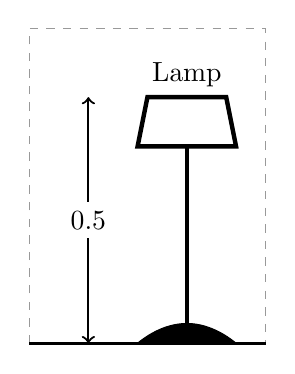
\begin{tikzpicture}
                \draw[dashed,white!60!black] (-2,0) rectangle (1,4);
                \draw[very thick] (-2,0) -- (1,0);
                \begin{scope}[scale=1.25]
                    %% labels
                    \draw[thick,<->] (-1,0) -- (-1,2.5) node[pos=0.5,anchor=center,fill=white] {\SI{0.5}{\meter}};
                    \node[anchor=south] at (0,2.5) {Lamp};
                    %% lamp
                    \draw[ultra thick] (-0.5,2) -- (-0.4,2.5) -- (0.4,2.5) -- (0.5,2) -- cycle;
                    \draw[ultra thick] (0,0) -- (0,2);
                    \draw[fill] (-0.5,0) parabola bend (0,0.2) (0.5,0) -- cycle;
                \end{scope}
            \end{tikzpicture}
        }
        \wrongchoice{
            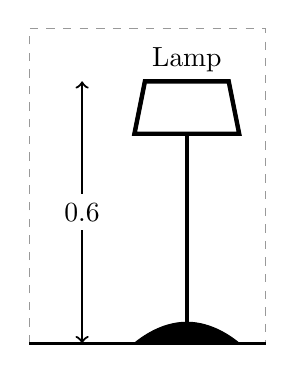
\begin{tikzpicture}
                \draw[dashed,white!60!black] (-2,0) rectangle (1,4);
                \draw[very thick] (-2,0) -- (1,0);
                \begin{scope}[scale=1.33]
                    %% labels
                    \draw[thick,<->] (-1,0) -- (-1,2.5) node[pos=0.5,anchor=center,fill=white] {\SI{0.6}{\meter}};
                    \node[anchor=south] at (0,2.5) {Lamp};
                    %% lamp
                    \draw[ultra thick] (-0.5,2) -- (-0.4,2.5) -- (0.4,2.5) -- (0.5,2) -- cycle;
                    \draw[ultra thick] (0,0) -- (0,2);
                    \draw[fill] (-0.5,0) parabola bend (0,0.2) (0.5,0) -- cycle;
                \end{scope}
            \end{tikzpicture}
        }
    \end{choices}
    \end{multicols}
\end{question}
}

\element{nysed}{
\begin{question}{June1995-Q91}
    Which type of image can be formed by a converging lens?
    \begin{choices}
        \wrongchoice{real images, only}
        \wrongchoice{virtual images, only}
      \correctchoice{both real and virtual images}
        \wrongchoice{neither real nor virtual images}
    \end{choices}
\end{question}
}

\element{nysed}{
\begin{question}{June1995-Q92}
    A converging lens is used to produce an image of an object.
    The object distance is twice the image distance.
    If the object is \SI{0.050}{\meter} tall,
        the height of its image is:
    \begin{multicols}{2}
    \begin{choices}
        \wrongchoice{\SI{0.010}{\meter}}
        \wrongchoice{\SI{0.020}{\meter}}
      \correctchoice{\SI{0.025}{\meter}}
        \wrongchoice{\SI{0.050}{\meter}}
    \end{choices}
    \end{multicols}
\end{question}
}

\element{nysed}{
\begin{question}{June1995-Q93}
    When an object is placed \SI{0.40}{\meter} from a diverging lens with a focal length of \SI{-0.10}{\meter},
        the image produced will be:
    \begin{choices}
      \correctchoice{virtual and smaller than the object}
        \wrongchoice{virtual and larger than the object}
        \wrongchoice{real and smaller than the object}
        \wrongchoice{real and larger than the object}
    \end{choices}
\end{question}
}

\element{nysed}{
\begin{question}{June1995-Q94}
    Photographers sometimes use colored filters to restrict the light entering a lens to a single wavelength.
    The filters are used to eliminate:
    \begin{choices}
        \wrongchoice{diffusion}
        \wrongchoice{diffraction}
        \wrongchoice{polarization effects}
      \correctchoice{chromatic aberration}
    \end{choices}
\end{question}
}

\element{nysed}{
\begin{question}{June1995-Q95}
    As an object is moved from \SI{0.2}{\meter} to \SI{0.3}{\meter} away from a plane mirror,
        the image distance:
    \begin{choices}
        \wrongchoice{decreases}
      \correctchoice{increases}
        \wrongchoice{remains the same}
    \end{choices}
\end{question}
}


%% Section June1994
%%--------------------
\element{nysed}{
\begin{question}{June1994-Q86}
    A plane mirror produces an image of an object.
    Compared to the object,
        the image appears:
    \begin{choices}
        \wrongchoice{inverted and the same size}
      \correctchoice{reversed and the same size}
        \wrongchoice{inverted and larger}
        \wrongchoice{reversed and larger}
    \end{choices}
\end{question}
}

\element{nysed}{
\begin{question}{June1994-Q87}
    A candle is located beyond the center of curvature, $C$, of a concave spherical mirror having principal focus, $F$, as shown in the diagram below.
    \begin{center}
    \begin{tikzpicture}
        %% Candle
        \draw[ultra thick,latex-] (-7,1) -- (-7,0) node[anchor=north] {Candle};
        %% labels
        \foreach \x/\y in {3/F,6/C} {
            \fill (-\x,0) circle (2pt) node[anchor=north] {$\y$};
        }
        %% mirror
        \draw (-8,0) -- (0,0);
        \draw[thick] (0,0) arc(0:{asin(1.5/6)}:6) node[anchor=south] {Mirror};
        \draw[thick] (0,0) arc(0:{-asin(1.5/6)}:6);
    \end{tikzpicture}
    \end{center}
    Where is the candle's image located?
    \begin{choices}
        \wrongchoice{beyond $C$}
      \correctchoice{beyond $C$ and $F$}
        \wrongchoice{between $F$ and the mirror}
        \wrongchoice{behind the mirror}
    \end{choices}
\end{question}
}

\element{nysed}{
\begin{question}{June1994-Q88}
    The convex spherical mirror found on the passenger side of many cars contains the warning: ``Objects are closer than they appear.''
    Which phrase best describes the image of an object viewed in this mirror?
    \begin{choices}
        \wrongchoice{real and smaller than the object}
        \wrongchoice{real and larger than the object}
      \correctchoice{virtual and smaller than the object}
        \wrongchoice{virtual and larger than the object}
    \end{choices}
\end{question}
}

\element{nysed}{
\begin{question}{June1994-Q89}
    A concave mirror with a focal length of \SI{20}{\centi\meter} is used to examine a \SI{0.50}{\centi\meter} wide freckle on a person's face.
    The person's face is located \SI{10}{\centi\meter} from the mirror.
    %% start question
    The image of the freckle produced by the mirror is:
    \begin{multicols}{2}
    \begin{choices}
        \wrongchoice{real and inverted}
        \wrongchoice{real and erect}
        \wrongchoice{virtual and inverted}
      \correctchoice{virtual and erect}
    \end{choices}
    \end{multicols}
\end{question}
}

\element{nysed}{
\begin{question}{June1994-Q90}
    A concave mirror with a focal length of \SI{20}{\centi\meter} is used to examine a \SI{0.50}{\centi\meter} wide freckle on a person's face.
    The person's face is located \SI{10}{\centi\meter} from the mirror.
    %% start question
    What is the width of the image of the freckle?
    \begin{multicols}{2}
    \begin{choices}
      \correctchoice{\SI{1.0}{\centi\meter}}
        \wrongchoice{\SI{2.0}{\centi\meter}}
        \wrongchoice{\SI{0.50}{\centi\meter}}
        \wrongchoice{\SI{1.5}{\centi\meter}}
    \end{choices}
    \end{multicols}
\end{question}
}

\element{nysed}{
\begin{question}{June1994-Q91}
    In the diagram below, a crown glass converging lens has foci $F$ and $F\prime$.
    An object is placed at a distance slightly less than the focal length from the lens,
        and a virtual image is produced.
    \begin{center}
    \begin{tikzpicture}
        %% principal axis
        \draw (-4,0) -- (4,0);
        \fill (-3,0) circle (2pt) node[anchor=north] {$F$};
        \fill (+3,0) circle (2pt) node[anchor=north] {$F\prime$};
        %% object
        \draw[ultra thick,-latex] (-2.5,0) -- (-2.5,1) node[anchor=south] {Object};
        %% lens
        \draw (0,1.5) arc ({180-asin(1.5/9)}:{180+asin(1.5/9)}:9);
        \draw (0,1.5) arc ({asin(1.5/9)}:{-asin(1.5/9)}:9);
        \node[anchor=west,text width=4em] at (0,1.5) {Crown glass lens};
    \end{tikzpicture}
    \end{center}
    The object remains in the same position and the crown glass lens is replaced with another lens of identical shape.
    If the new lens produces a real image of the object,
        the new lens is most likely made of:
    \begin{multicols}{2}
    \begin{choices}
        \wrongchoice{water}
        \wrongchoice{Lucite}
        \wrongchoice{fused quartz}
      \correctchoice{flint glass}
    \end{choices}
    \end{multicols}
\end{question}
}

\element{nysed}{
\begin{question}{June1994-Q92}
    Which diagram below shows the path of light rays as they pass from an object at $2F$ through a converging lens to the image formed at $2F\prime$?
    \begin{choices}
        \AMCboxDimensions{down=-1.2cm}
        %% ANS is 1
        \correctchoice{
            \begin{tikzpicture}
                %% principal axis
                \draw (-3.2,0) -- (3.2,0);
                %% left labels
                \foreach \x/\y in {1.5/F,3/2F}
                    \fill (-\x,0) circle (2pt) node[anchor=south] {$\y\prime$};
                %% right labels
                \foreach \x/\y in {1.5/F,3/2F}
                    \fill (+\x,0) circle (2pt) node[anchor=north] {$\y$};
                %% lens
                \draw (0,1.5) arc ({180-asin(1.5/4.5)}:{180+asin(1.5/4.5)}:4.5);
                \draw (0,1.5) arc ({asin(1.5/4.5)}:{-asin(1.5/4.5)}:4.5);
                \draw[dashed] (0,1.5) -- (0,-1.5);
                %% object
                \draw[very thick,-latex] (+3,0) -- (+3,1) node[anchor=south] {Object};
                \begin{scope}[decoration={markings,mark=at position 0.66 with {\arrow{latex}}}]
                    \draw[thick,postaction={decorate}] (3,1)  -- (0,0);
                    \draw[thick,postaction={decorate}] (0,0)  -- (-3,-1);
                    \draw[thick,postaction={decorate}] (3,1)  -- (0,-1);
                    \draw[thick,postaction={decorate}] (0,-1)  -- (-3,-1);
                \end{scope}
                %% image
                \draw[very thick,-latex] (-3,0) -- (-3,-1);
            \end{tikzpicture}
        }
        \wrongchoice{
            \begin{tikzpicture}
                %% principal axis
                \draw (-3.2,0) -- (3.2,0);
                %% left labels
                \foreach \x/\y in {1.5/F,3/2F}
                    \fill (-\x,0) circle (2pt) node[anchor=south west] {$\y\prime$};
                %% right labels
                \foreach \x/\y in {1.5/F,3/2F}
                    \fill (+\x,0) circle (2pt) node[anchor=north] {$\y$};
                %% lens
                \draw (0,1.5) arc ({180-asin(1.5/4.5)}:{180+asin(1.5/4.5)}:4.5);
                \draw (0,1.5) arc ({asin(1.5/4.5)}:{-asin(1.5/4.5)}:4.5);
                \draw[dashed] (0,1.5) -- (0,-1.5);
                %% object
                \draw[very thick,-latex] (+3,0) -- (+3,1) node[anchor=south] {Object};
                \begin{scope}[decoration={markings,mark=at position 0.66 with {\arrow{latex}}}]
                    \draw[thick,postaction={decorate}] (3,1)  -- (45:2ex);
                    \draw[thick,postaction={decorate}] (45:2ex) -- (225:2ex);
                    \draw[thick,postaction={decorate}] (225:2ex)  -- (-3,-1);
                    \draw[thick,postaction={decorate}] (3,0)  -- (0,1);
                    \draw[thick,postaction={decorate}] (0,1)  -- (-3,1) -- (-3,0);
                \end{scope}
                %% image
                \draw[very thick,-latex] (-3,0) -- (-3,-1);
            \end{tikzpicture}
        }
        \wrongchoice{
            \begin{tikzpicture}
                %% principal axis
                \draw (-3.2,0) -- (3.2,0);
                %% left labels
                \foreach \x/\y in {1.5/F,3/2F}
                    \fill (-\x,0) circle (2pt) node[anchor=south] {$\y\prime$};
                %% right labels
                \foreach \x/\y in {1.5/F,3/2F}
                    \fill (+\x,0) circle (2pt) node[anchor=north] {$\y$};
                %% lens
                \draw (0,1.5) arc ({180-asin(1.5/4.5)}:{180+asin(1.5/4.5)}:4.5);
                \draw (0,1.5) arc ({asin(1.5/4.5)}:{-asin(1.5/4.5)}:4.5);
                \draw[dashed] (0,1.5) -- (0,-1.5);
                %% object
                \draw[very thick,-latex] (+3,0) -- (+3,1) node[anchor=south] {Object};
                \begin{scope}[decoration={markings,mark=at position 0.5 with {\arrow{latex}}}]
                    \draw[thick,postaction={decorate}] (3,1)  -- (0,1);
                    \draw[thick,postaction={decorate}] (0,1)  -- (-3,0);
                    \draw[thick,postaction={decorate}] (3,1)  -- (45:2ex);
                    \draw[thick,postaction={decorate}] (45:2ex) -- (225:2ex);
                    \draw[thick,postaction={decorate}] (225:2ex)  -- (-3,-1);
                \end{scope}
                %% image
                \draw[very thick,-latex] (-3,0) -- (-3,-1);
            \end{tikzpicture}
        }
        \wrongchoice{
            \begin{tikzpicture}
                %% principal axis
                \draw (-3.2,0) -- (3.2,0);
                %% left labels
                \foreach \x/\y in {1.5/F,3/2F}
                    \fill (-\x,0) circle (2pt) node[anchor=south] {$\y\prime$};
                %% right labels
                \foreach \x/\y in {1.5/F,3/2F}
                    \fill (+\x,0) circle (2pt) node[anchor=north] {$\y$};
                %% lens
                \draw (0,1.5) arc ({180-asin(1.5/4.5)}:{180+asin(1.5/4.5)}:4.5);
                \draw (0,1.5) arc ({asin(1.5/4.5)}:{-asin(1.5/4.5)}:4.5);
                \draw[dashed] (0,1.5) -- (0,-1.5);
                %% object
                \draw[very thick,-latex] (+3,0) -- (+3,1) node[anchor=south] {Object};
                \begin{scope}[decoration={markings,mark=at position 0.66 with {\arrow{latex}}}]
                    \draw[thick,postaction={decorate}] (3,1)  -- (0,-1);
                    \draw[thick,postaction={decorate}] (0,-1)  -- (-3,0);
                    \draw[thick,postaction={decorate}] (3,1)  -- (45:2ex);
                    \draw[thick,postaction={decorate}] (45:2ex) -- (225:2ex);
                    \draw[thick,postaction={decorate}] (225:2ex)  -- (-3,-1);
                \end{scope}
                %% image
                \draw[very thick,-latex] (-3,0) -- (-3,-1);
            \end{tikzpicture}
        }
    \end{choices}
\end{question}
}

\element{nysed}{
\begin{question}{June1994-Q93}
    A student placed an object at various distances ($d_0$) from a converging lens.
    The corresponding image distance ($d_i$) was measured and recorded in the data below.
    \begin{center}
    \begin{tabular}{cccc}
        \toprule
        $d_0$ & \SI{0.15}{\meter} & \SI{0.20}{\meter} & \SI{0.30}{\meter} \\
        $d_i$ & \SI{0.30}{\meter} & \SI{0.20}{\meter} & \SI{0.15}{\meter} \\
        \bottomrule
    \end{tabular}
    \end{center}
    What is the focal length of the lens?
    \begin{multicols}{2}
    \begin{choices}
      \correctchoice{\SI{0.10}{\meter}}
        \wrongchoice{\SI{0.15}{\meter}}
        \wrongchoice{\SI{0.20}{\meter}}
        \wrongchoice{\SI{0.30}{\meter}}
    \end{choices}
    \end{multicols}
\end{question}
}

\element{nysed}{
\begin{question}{June1994-Q94}
    A lens forms a real image three times the size of the object when the image is \SI{0.12}{\meter} from the lens.
    How far from the lens is the object?
    \begin{multicols}{2}
    \begin{choices}
        \wrongchoice{\SI{0.36}{\meter}}
        \wrongchoice{\SI{0.09}{\meter}}
        \wrongchoice{\SI{0.03}{\meter}}
      \correctchoice{\SI{0.04}{\meter}}
    \end{choices}
    \end{multicols}
\end{question}
}

\element{nysed}{
\begin{question}{June1994-Q95}
    What causes chromatic aberration in a crown glass lens?
    \begin{choices}
        \wrongchoice{Each wavelength of light reflects from the surface of the lens}
      \correctchoice{Each wavelength of light is refracted a different amount by the lens}
        \wrongchoice{White light waves interfere inside the lens}
        \wrongchoice{White light waves diffracted around the edge of the lens}
    \end{choices}
\end{question}
}


%% Section June1986
%%--------------------
\element{nysed}{
\begin{question}{June1986-Q28}
    Which diagram best represents the image of the letter ``L'' formed by the plane mirror $MM\prime$?
    \begin{center}
    \begin{tikzpicture}
        %% Letter L
        \draw[very thick] (-2,2) -- (-2,0) -- (-1,0);
        %% Mirror MM\prime
        \draw (0,3) -- (0,-1);
        \node[anchor=south] at (0,+3) {$M\prime$};
        \node[anchor=north] at (0,-1) {$M$};
    \end{tikzpicture}
    \end{center}
    \begin{multicols}{2}
    \begin{choices}
        \AMCboxDimensions{down=-1.2cm}
        \wrongchoice{
            \begin{tikzpicture}
                \draw[dashed,white!50!black] (-1.5,-1.5) rectangle (1.5,1.5);
                \draw[very thick] (0.5,1) -- (-0.5,1) -- (-0.5,-1);
            \end{tikzpicture}
        }
        \wrongchoice{
            \begin{tikzpicture}
                \draw[dashed,white!50!black] (-1.5,-1.5) rectangle (1.5,1.5);
                \draw[very thick] (-0.5,1) -- (0.5,1) -- (0.5,-1);
            \end{tikzpicture}
        }
        \wrongchoice{
            \begin{tikzpicture}
                \draw[dashed,white!50!black] (-1.5,-1.5) rectangle (1.5,1.5);
                \draw[very thick] (-0.5,1) -- (-0.5,-1) -- (0.5,-1);
            \end{tikzpicture}
        }
        %% ANS is 4
        \correctchoice{
            \begin{tikzpicture}
                \draw[dashed,white!50!black] (-1.5,-1.5) rectangle (1.5,1.5);
                \draw[very thick] (0.5,1) -- (0.5,-1) -- (-0.5,-1);
            \end{tikzpicture}
        }
    \end{choices}
    \end{multicols}
\end{question}
}

\newcommand{\nysedJuneNineteenEightySixQEightyFive}{
\begin{tikzpicture}[scale=0.9]
    \draw[thick,-latex] (-4.2,0) -- (4.2,0);
    %% lens
    \draw (0,1.5) arc({asin(1.5/6)}:{-asin(1.6/6)}:6);
    \draw (0,1.5) arc({180-asin(1.5/6)}:{180+asin(1.6/6)}:6);
    %% object
    \draw[very thick,-latex] (-4,0) -- (-4,1);
    \draw (0,-0.1) -- (0,0.1) node[anchor=south] {$A$};
    %% labels
    \foreach \x/\y in {-4/O,-3/B,-2/F,-1/D,2/F\prime,4/2F\prime}
        \draw (\x,0.1) -- (\x,-0.1) node[anchor=north] {$\y$};
\end{tikzpicture}
}

\element{nysed}{
\begin{question}{June1986-Q85}
    The diagram below represents an object placed at point $O$,
        located \SI{1.0}{\meter} from a lens of focal length \SI{0.5}{\meter}.
    \begin{center}
        \nysedJuneNineteenEightySixQEightyFive
    \end{center}
    The distance between the lens and the image is:
    \begin{multicols}{2}
    \begin{choices}
      \correctchoice{\SI{1.0}{\meter}}
        \wrongchoice{\SI{0.50}{\meter}}
        \wrongchoice{\SI{0.25}{\meter}}
        \wrongchoice{\SI{1.5}{\meter}}
    \end{choices}
    \end{multicols}
\end{question}
}

\element{nysed}{
\begin{question}{June1986-Q86}
    The diagram below represents an object placed at point $O$,
        located \SI{1.0}{\meter} from a lens of focal length \SI{0.5}{\meter}.
    \begin{center}
        \nysedJuneNineteenEightySixQEightyFive
    \end{center}
    Compared to the size of the object,
        the size of the image is:
    \begin{multicols}{3}
    \begin{choices}
        \wrongchoice{smaller}
        \wrongchoice{larger}
      \correctchoice{the same}
    \end{choices}
    \end{multicols}
\end{question}
}

\element{nysed}{
\begin{question}{June1986-Q87}
    The diagram below represents an object placed at point $O$,
        located \SI{1.0}{\meter} from a lens of focal length \SI{0.5}{\meter}.
    \begin{center}
        \nysedJuneNineteenEightySixQEightyFive
    \end{center}
    Compared to the image when the object is at point $O$,
        the image when the object is moved to point $B$ will be:
    \begin{choices}
        \wrongchoice{smaller}
        \wrongchoice{changed from inverted to erect}
        \wrongchoice{nearer the lens}
      \correctchoice{farther from the lens}
    \end{choices}
\end{question}
}

\element{nysed}{
\begin{question}{June1986-Q88}
    The diagram below represents an object placed at point $O$,
        located \SI{1.0}{\meter} from a lens of focal length \SI{0.5}{\meter}.
    \begin{center}
        \nysedJuneNineteenEightySixQEightyFive
    \end{center}
    The original lens is replaced with one having a shorter focal length.
    If the object remains at point $O$,
        compared to the original image distance, the new image distance:
    \begin{choices}
      \correctchoice{is smaller}
        \wrongchoice{is larger}
        \wrongchoice{remains the same}
    \end{choices}
\end{question}
}


%% Section June1985
%%--------------------
\element{nysed}{
\begin{question}{June1985-Q27}
    The image formed by a diverging lens is:
    \begin{multicols}{2}
    \begin{choices}
        \wrongchoice{enlarged}
        \wrongchoice{inverted}
        \wrongchoice{real}
      \correctchoice{virtual}
    \end{choices}
    \end{multicols}
\end{question}
}


\endinput


